% Chapter 1

\chapter{Introducción General} % Main chapter title

\label{Chapter1} % For referencing the chapter elsewhere, use \ref{Chapter1} 
\label{IntroGeneral}

%----------------------------------------------------------------------------------------

% Define some commands to keep the formatting separated from the content 
\newcommand{\keyword}[1]{\textbf{#1}}
\newcommand{\tabhead}[1]{\textbf{#1}}
\newcommand{\code}[1]{\texttt{#1}}
\newcommand{\file}[1]{\texttt{\bfseries#1}}
\newcommand{\option}[1]{\texttt{\itshape#1}}
\newcommand{\grados}{$^{\circ}$}

%----------------------------------------------------------------------------------------

%\section{Introducción}

%----------------------------------------------------------------------------------------
\section{Aprendiendo \LaTeX{}}

\LaTeX{} no es \textsc{WYSIWYG} (What You See is What You Get), a diferencia de los procesadores de texto como Microsoft Word o Pages de Apple o incluso LibreOffice en el mundo open-source. En lugar de ello, un documento escrito para \LaTeX{} es en realidad un archivo de texto simple, llano que \emph{no contiene formato} . Nosotros le decimos a \LaTeX{} cómo deseamos que se aplique el formato en el documento final escribiendo comandos simples entre el texto, por ejemplo, si quiero usar \emph{texto en cursiva para dar énfasis}, escribo \verb|\emph{texto}| y pongo el texto en cursiva que quiero entre medio de las llaves. Esto significa que \LaTeX{} es un lenguaje del tipo \enquote{mark-up}, muy parecido a HTML.

\subsection{Una introducción (no tan corta) a \LaTeX{}}

Si usted es nuevo a \LaTeX{}, hay un muy buen libro electrónico - disponible gratuitamente en Internet como un archivo PDF - llamado, \enquote{A (not so short) Introduction to \LaTeX{}}. El título del libro es generalmente acortado a simplemente \emph{lshort}. Puede descargar la versión más reciente en inglés (ya que se actualiza de vez en cuando) desde aquí:
\url{http://www.ctan.org/tex-archive/info/lshort/english/lshort.pdf}

Está disponible en varios idiomas además del inglés. Se puede encontrar la versión en español en la lista en esta página: \url{http://www.ctan.org/tex-archive/info/lshort/}


\subsection{Guía matemática rápida para \LaTeX{}}

Si usted está escribiendo un documento con mucho contenido matemático, entonces es posible que desee leer el documento de la AMS (American Mathematical Society) llamado, \enquote{A Short Math Guide for \LaTeX{}}. Se puede encontrar en línea en el siguiente link: \url{http://www.ams.org/tex/amslatex.html} en la sección \enquote{Additional Documentation} hacia la parte inferior de la página.


%----------------------------------------------------------------------------------------

\section{Utilizando esta plantilla}

Si usted está familiarizado con \LaTeX{}, entonces puede explorar la estructura de directorios de esta plantilla y proceder a personalizarla agregando su información en el bloque \emph{INFORMACIÓN DE LA PORTADA} en el archivo \file{memoria.tex}.  

Se puede continuar luego modificando el resto de los archivos siguiendo los lineamientos que se describen en la sección \ref{sec:FillingFile} en la página \pageref{sec:FillingFile}.

Asegúrese de leer el capítulo \ref{Chapter2} acerca de las convenciones utilizadas para las Memoria de los Trabajos Finales de la Carrera de Especialización en Sistemas Embebidos de FIUBA.

Si es nuevo en \LaTeX{} se recomienda que continue leyendo el documento ya que contiene información básica para aprovechar el potencial de esta herramienta.


\subsection{Acerca de esta plantilla}

Esta plantilla \LaTeX{} está basada originalmente en torno a un archivo de estilo \LaTeX{} creado por Steve R.\ Gunn de la  University of Southampton (UK), department of Electronics and Computer Science. Se puede encontrar su trabajo original en el siguiente sitio de internet:
\url{http://www.ecs.soton.ac.uk/~srg/softwaretools/document/templates/}

El archivo de Gunn, \file{ecsthesis.cls} fue posteriormente modificado por Sunil Patel quien creó una plantilla esqueleto con la estructura de carpetas. El template resultante se puede encontrar en el sitio web de Sunil Patel:
\url{http://www.sunilpatel.co.uk/thesis-template}

El template de Patel se publicó a través de  \url{http://www.LaTeXTemplates.com} desde donde fue modificado muchas veces en base a solicitudes de usuarios. La versión 2.0 y subsiguientes representan cambios significativos respecto a la versión de la plantilla modificada por Patel, que es de hecho, dificilmente reconocible. El trabajo en la version 2.0 fue realizado por Vel Gayevskiy y Johannes Böttcher.

Uno de los primeros graduados de la Carerra de Especialización en Sistemas Embebios de la UBA, el Ing. \href{mailto:pbos@fi.uba.ar}{Patricio Bos} modificó los contenidos de la versión 2.3 para crear una plantilla altamente adaptada a la Carrera de Especialización de la UBA.

%----------------------------------------------------------------------------------------

\section{Qué incluye esta plantilla}

\subsection{Carpetas}

Esta plantilla se distribuye como una único archivo .zip que se puede descomprimir en varios archivos y carpetas. Los nombres de las carpetas son (o pretender ser) auto-explicativos.

\keyword{Appendices} -- Esta es la carpeta donde se deben poner los apéndices. Cada apéndice debe ir en su propio archivo \file{.tex}. Se incluye un ejemplo y una plantilla en la carpeta.

\keyword{Chapters} -- Esta es la carpeta donde se deben poner los capítulos de la memoria. Cada capítulo debe ir un su propio archivo \file{.tex} por separado.  Se ofrece por defecto, la siguiente estructura de capítulos y se recomienda su utilización dentro de lo posible:

\begin{itemize}
\item Capítulo 1: Introducción general	
\item Capítulo 2: Introducción específica
\item Capítulo 3: Diseño e implementación
\item Capítulo 4: Ensayos y resultados
\item Capítulo 5: Conclusiones

\end{itemize}

Esta estructura de capítulos es la que se recomienda para las memorias de la especialización.

\keyword{Figures} -- Esta carpeta contiene todas las figuras de la memoria.  Estas son las versiones finales de las imágenes que van a ser incluidas en la memoria.  Pueden ser imágenes en formato \textit{raster}\footnote{\url{https://en.wikipedia.org/wiki/Raster_graphics}} como \file{.png}, \file{.jpg} o en formato vectoriales\footnote{\url{https://en.wikipedia.org/wiki/Vector_graphics}} como \file{.pdf}, \file{.ps}.  Se debe notar que utilizar imágenes vectoriales disminuye notablemente el peso del documento final y acelera el tiempo de compilación por lo que es recomendable su utilización siempre que sea posible.

\subsection{Archivos}

También están incluidos varios archivos, la mayoría de ellos son de texto plano y se puede ver su contenido en un editor de texto. Después de la compilación inicial, se verá que más archivos auxiliares son creados por \ LaTeX{} o BibTeX, pero son de uso interno y que no es necesario eliminarlos o hacer nada con ellos.  Toda la información necesaria para complilar el documento se encuentra en los archivos \file{.tex} y en las imágenes de la carpeta Figures.

\keyword{referencias.bib} - este es un archivo importante que contiene toda la información bibliográfica y de referencias que se utilizará para las citas en la memoria en conjunto con BibTeX. Usted puede escribir las entradas bibliográficas en forma manual, aunque existen también programas de gestión de referencias que facilitan la creación y gestión de las referencias y permiten exportarlas en formato BibTeX.  También hay disponibles sitios web como \url{books.google.com} que permiten obtener toda la información necesaria para una cita en formato BibTeX.

\keyword{MastersDoctoralThesis.cls} -- este es un archivo importante. Es el archivos con la clase que le informa a \LaTeX{} cómo debe dar formato a la memoria. El usuario de la plantilla no debería necesitar modificar nada de este archivo.

\keyword{memoria.pdf} -- esta es su memoria con una tipografía bellamente compuesta (en formato de archivo PDF) creado por \LaTeX{}. Se distribuye con la plantilla y después de compilar por primera vez sin hacer ningún cambio se debería obtener una versión idéntica a este documento.

\keyword{memoria.tex} -- este es un archivo importante. Este es el archivo que tiene que compilar \LaTeX{} para producir la memoria como un archivo PDF. Contiene un marco de trabajo y estructuras que le indican a \LaTeX{} cómo diagramar la memoria.  Está altamente comentado para que se pueda entender qué es lo que realiza cada línea de código y por qué está incluida en ese lugar.  En este archivo se debe completar la información personalizada de las primeras sección según se indica en la sección \ref{sec:FillingFile}.

Archivos que \emph{no} forman parte de la distribución de la plantilla pero que son generados por \LaTeX{} como archivos auxiliares necesarios para la producción de la memoria.pdf son:

\keyword{memoria.aux} -- este es un archivo auxiliar generado por \LaTeX{}, si se borra \LaTeX{} simplemente lo regenera cuando se compila el archivo principal \file{memoria.tex}.

\keyword{memoria.bbl} -- este es un archivo auxiliar generado por BibTeX, si se borra BibTeX simplemente lo regenera cuando se compila el archivo principal \file{memoria.tex}. Mientras que el archivo \file{.bib} contiene todas las referencias que hay, este archivo \file{.bbl} contine sólo las referencias que han sido citadas y se utiliza para la construcción de la bibiografía.

\keyword{memoria.blg} -- este es un archivo auxiliar generado por BibTeX, si se borra BibTeX simplemente lo regenera cuando se compila el archivo principal \file{memoria.tex}.

\keyword{memoria.lof} -- este es un archivo auxiliar generado por \LaTeX{}, si se borra \LaTeX{} simplemente lo regenera cuando se compila el archivo principal \file{memoria.tex}.  Le indica a \LaTeX{} cómo construir la sección \emph{Lista de Figuras}.
 
\keyword{memoria.log} --  este es un archivo auxiliar generado por \LaTeX{}, si se borra \LaTeX{} simplemente lo regenera cuando se compila el archivo principal \file{memoria.tex}. Contiene mensajes de \LaTeX{}. Si se reciben errores o advertencias durante la compilación, se guardan en este archivo \file{.log}.

\keyword{memoria.lot} -- este es un archivo auxiliar generado por \LaTeX{}, si se borra \LaTeX{} simplemente lo regenera cuando se compila el archivo principal \file{memoria.tex}.  Le indica a \LaTeX{} cómo construir la sección \emph{Lista de Tablas}.

\keyword{memoria.out} -- este es un archivo auxiliar generado por \LaTeX{}, si se borra \LaTeX{} simplemente lo regenera cuando se compila el archivo principal \file{memoria.tex}.

De esta larga lista de archivos, sólo aquellos con la extensión \file{.bib}, \file{.cls} y \file{.tex} son importantes.  Los otros archivos auxiliares pueden ser ignorados o borrados ya que \LaTeX{} y BibTeX los regenerarán durante la compilación.

%----------------------------------------------------------------------------------------

\section{Entorno de trabajo}

Ante de comenzar a editar la plantilla debemos tener un editor \LaTeX{} instalado en nuestra computadora.  En forma análoga a lo que sucede en lenguaje C, que se puede crear y editar código con casi cualquier editor, exiten ciertos entornos de trabajo que nos pueden simplificar mucho la tarea.  En este sentido, se recomienda, sobre todo para los principiantes en \LaTeX{} la utilización de TexMaker, un programa gratuito y multi-plantaforma que está disponible tanto para windows como para sistemas GNU/linux.

La versión más reciente de TexMaker es la 4.5 y se puede descargar del siguiente link: \url{http://www.xm1math.net/texmaker/download.html}. Se puede consultar el manual de usuario en el siguiente link: \url{http://www.xm1math.net/texmaker/doc.html}.

\subsection{Configurando TexMaker}

La instalación de TexMaker se encarga de instalar todos los paquetes necesarios de \LaTeX{}. 
Una vez instalado el programa y abierto el archivo memoria.tex se debería ver una pantalla similar a la figura \ref{fig:texmaker}. 

\begin{figure}[h]
	\centering
	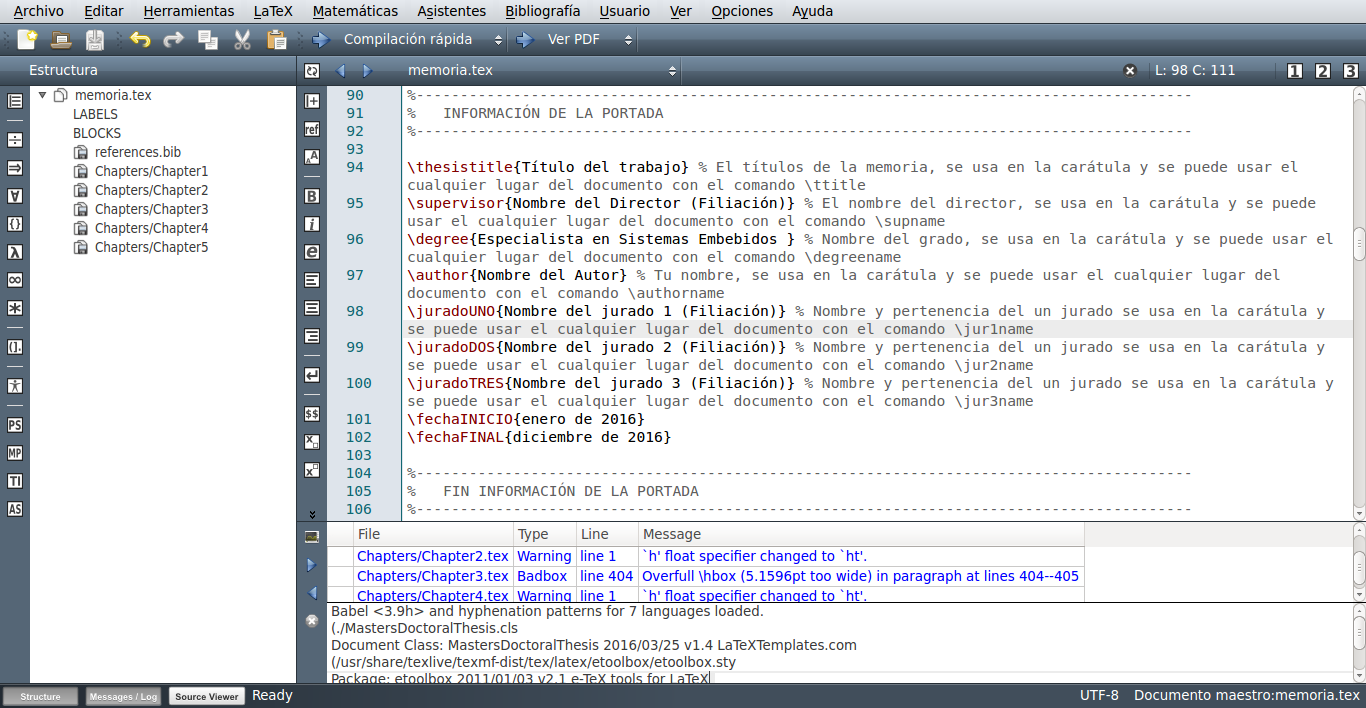
\includegraphics[width=\textwidth]{./Figures/texmaker.png}
	\caption{Entorno de trabajo del texMaker.}
	\label{fig:texmaker}
\end{figure}

Notar que existe una vista llamada Estructura a la izquierda de la interface que nos permite abrir desde dentro del programa los archivos individuales de los capítulos.  A la derecha se encuentra una vista con el archivo propiamente dicho para su edición. Hacia la parte inferior se encuentra una vista del log con información de los resultados de la compilación.  En esta última vista pueden aparecen advertencias o \textit{warning} que normalmente pueden ser ignorados y también los errores que se indican en color rojo.

Recordar que el archivo que se debe compilar con PDFLaTex es \file{memoria.tex}, si trataramos de compilar alguno de los capítulos directamente nos saldría un error.  Para salvar la molestia de tener que cambiar de archivo para compilar, se puede definer el archivo \file{memoria.tex} como ``documento maestro'' yendo al menú opciones -> ``definir documento actual como documento maestro'', lo que nos permite compilar cualquier archivo, sea memoria.tex, el capítulo donde estemos trabajando o incluso un apéndice si lo hubiera y texmaker se encargará automáticamente de compilar memoria.tex.

En el menú herramientas se encuentran las opciones de compilación.  Para producir un archivo PDF a partir de un archivo .tex se debe ejecutar PDFLaTeX (el shortcut es F6). Para incorporar nueva bibliografía se debe utilizar la opción BibTeX del mismo menú herramientas (el shortcut es F11).

Notar que para actualizar las tablas de contenidos se debe ejecutar PDFLaTeX dos veces.  Esto se debe a que es necesario actualizar algunos archivos auxiliares antes de obtener el resultado final.  En forma similar, para actualizar las referecias se debe ejecutar primero PDFLaTeX, después BibTeX y finalmente PDFLaTeX dos veces por idénticos motivos.

\section{Personalizando la plantilla en el archivo \file{memoria.tex}}
\label{sec:FillingFile}

Para personalizar la plantilla se debe incorporar la información propia en los distintos archivos \file{.tex}. 

Primero abrir \file{memoria.tex} con TexMaker (o el editor de su preferencia). Se debe ubicar dentro del archivo el bloque de código titulado \emph{INFORMACIÓN DE LA PORTADA} donde se deben incorporar los primeros datos personales con los que se constuirá automáticamente la portada.


%----------------------------------------------------------------------------------------

\section{El código del archivo \file{memoria.tex} explicado}

El archivo \file{memoria.tex} contiene la estructura de la memoria y se encuentra densamente comentado para explicar qué páginas, secciones y elementos de formato el código \LaTeX{} está creando en cada línea. Cada elemento de mayor jerarquía del documento está dividido en bloques con nombres en mayúsculas para que resulte evidente qué es lo que hace esa porción de código en particular. Inicialmente puede parecer que hay mucho código \LaTeX{}, pero es principalmente código para dar formato a la memoria y al estar ya definido, no requiere intervención del usuario de la plantilla.

Se debe comenzar por chequear que la información en la portada es correcta.

Luego viene el resumen que contiene una versión abreviada de su trabajo.  Se debería poder utilizar como un documento independiente para describir el contenido de su trabajo.

A continuación se encuentra la sección opcional de agradecimientos. 

El índice de contenidos, las listas de figura de tablas se generan en forma automática y no requieren intervención ni edición manual por parte del usuario de la plantilla. 

La siguiente página es opcional y puede contener una dedicatorio de una línea, en caso de que usted quiere dedicarle el trabajo a alguien.

Finalmente, se encuentra el bloque donde se incluyen los capítulos y los apéndices.  Por defecto se incluyen los 5 capítulos propuestos que se encuentran en la carpeta /Chapters. Cada capítulo se debe escribir en un archivo .tex separado y se debe poner en la carpeta \emph{Chapters} con el nombre \file{Chapter1}, \file{Chapter2}, etc\ldots El código para incluir capítulos desde archivos externos se muestra a continuación.

\begin{verbatim}
	% Chapter 1

\chapter{Introducción General} % Main chapter title

\label{Chapter1} % For referencing the chapter elsewhere, use \ref{Chapter1} 
\label{IntroGeneral}

%----------------------------------------------------------------------------------------

% Define some commands to keep the formatting separated from the content 
\newcommand{\keyword}[1]{\textbf{#1}}
\newcommand{\tabhead}[1]{\textbf{#1}}
\newcommand{\code}[1]{\texttt{#1}}
\newcommand{\file}[1]{\texttt{\bfseries#1}}
\newcommand{\option}[1]{\texttt{\itshape#1}}
\newcommand{\grados}{$^{\circ}$}

%----------------------------------------------------------------------------------------

\section{Introducción}

%----------------------------------------------------------------------------------------

\section{Producción de vino}


\section{Motivación}

En el presente trabajo se busca satisfacer las necesidades de la bodega de mi primo. La cual se necesita controlar un proceso delicado como es la fermentación del vino y se requiere un cuidado continúo. Por el momento es realizado por personal día y noche. Teniendo en cuenta que en la zona de trabajo es difícil conseguir personas responsables que se comprometan con el trabajo. 

A su vez se busca también una satisfaccion personal, dado que hacía tiempo que buscaba poder implementar en un microtrolador una interfaz que permita visualizar la información de un sistema mediante una plataforma web, donde se pueda apreciar el estado de las entradas y poder ejercer control sobre ellas.

Y para concluir, el hecho de utilizar la plataforma CIAA, la cual me permitió cumplir todo estos objetivos, haciendo uso de un sitema operativo de tiempo real (RTOS), como sé llamará de aqui en adelante.



\section{Proyecto CIAA}

\section{Objetivos y Alcances}






	\chapter{Introducción Específica} % Main chapter title

\label{Chapter2}
%
%%----------------------------------------------------------------------------------------
%%	SECTION 1
%%----------------------------------------------------------------------------------------
%La idea de esta sección es presentar el tema de modo que cualquier persona que no conoce el tema pueda entender de qué se trata y por qué es importante realizar este trabajo y cuál es su impacto.
%\label{sec:ejemplo}
En este sección se detallaran las tareas que se realizaron, que contratiempos se tuvieron y cuales fueron los requerimientos.

\section{Objetivos y alcances}

\subsection*{Objetivos}
    Desarrollar un software que permiea controlar, monitorear y supervisar el proceso de fermentación del vino en las bodegas en forma automática. Aprovechando el proyecto CIAA, se utilizó esta plataforma ya que está preparada especialmente para aplicaciones industriales, siendo esta libre y gratuita.
\subsection*{Alcance}
  \begin{itemize}
      \item Sensar la temepratura de un tanque de fermentacion de ya se para vinos tintos o blancos.
      \item Controlar que la temperatura se mantenga dentro del rango correspondiente según el tipo de vino. 
      \item En caso de corte de energia se notificar vía SMS a un celuar de contacto.
      \item Mensajes de alerta vía SMS en caso de temperatura fuera de rango.
      \item Diseño de una página que permita mostrar la informacion del sistema y realizar las configuraciones necesarias.
      \item Diseño de una placa básica para mostrar el funcionamiento del sitema.
  \end{itemize}

  \section{Requerimientos}

Estos fueron consensuados con el responable de la Bodega Chico Zossi, para trabajar sobre un caso real. 

\begin{enumerate}[label*=\arabic*.]
  \item Medición de Temperatura:
    \begin{enumerate}[label*=\arabic*.]
      \item  Se requiere medir la temperatura de un tanques.
      \item La resolución de debe ser de $\pm 1^oC$.
    \end{enumerate}
  \item Comunicación:
    \begin{enumerate}[label*=\arabic*.]
      \item Debe poder transmitir mensajes SMS notificando el estado/cambios producidos.
      \item Acceso web para la configuración de los parámetros requeridos de temperatura. 
    \end{enumerate}
  \item Funcionamiento del Sistema embebido:
    \begin{enumerate}[label*=\arabic*.]
      \item El sistema deberá mantener la temperatura controlada a los parámetros configurados por el usuario. Para ello deberá hacer uso del actuadores.
      \item Deberá alertar si hay corte de energía mediante un SMS.
      \item Deberá mostrar el nivel de batería.
  \end{enumerate}
\end{enumerate}


\section{Desglose de tareas - GANTT}
Para llevar el proyecto a cabo se desarrollo la siguiente planificación de tareas y se estimaron que tiempos debían emplearse para cada una de ellas.

A su vez se analizaron que tareas debian realizarse primero y cuales eran sus dependencias. De esta forma, si se presentara alguna complicacion poder tener un análisis mas completo de como podria esto afectar a la fecha de entrega del proyecto.

Todo este estudio fue aprovechado de haber realizado la asignatura de Gestion de Proyectos. Podemos ver en la siguiente figura \ref{fig:gantt} el plan de trabajo.

\begin{landscape}
  \pagestyle{empty}
  \begin{figure}[htb]
      \centering
      %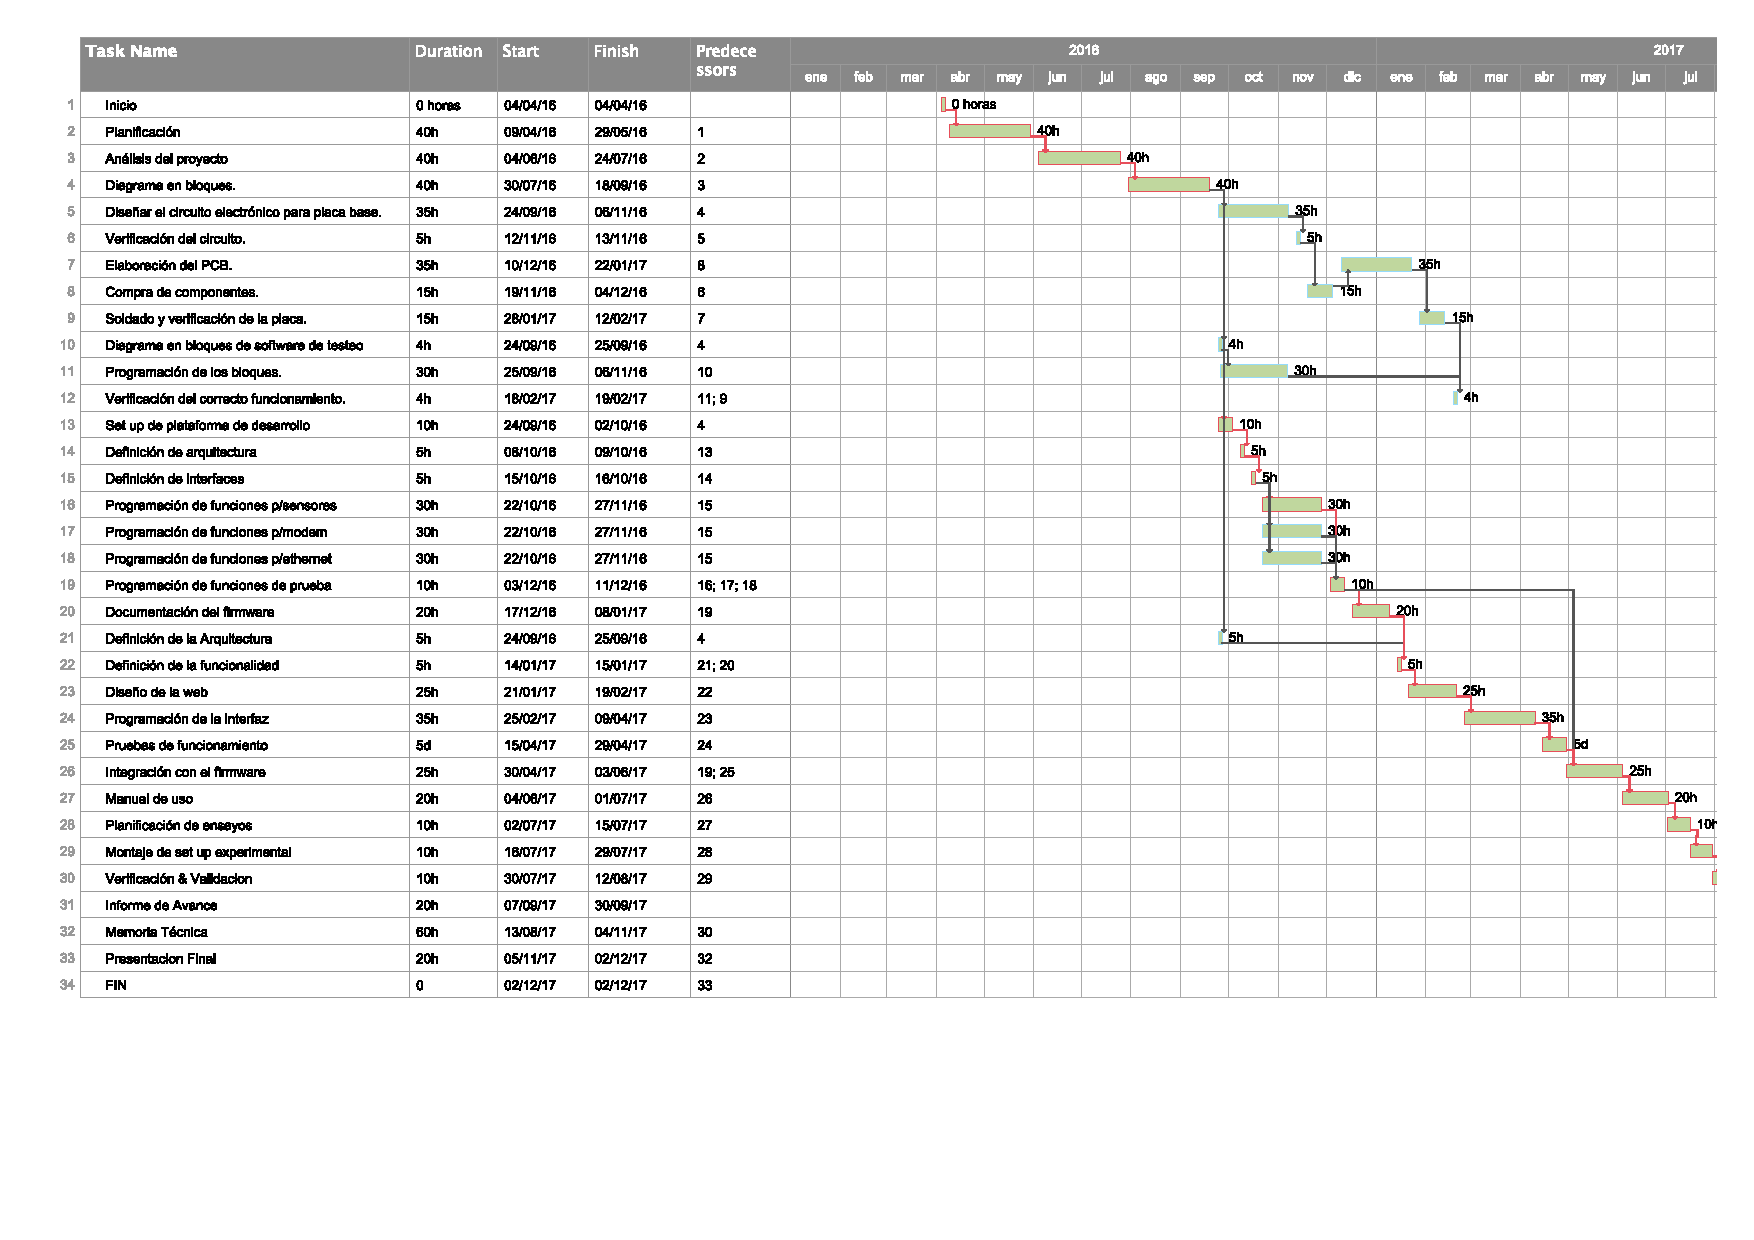
\includegraphics[page=1,clip, trim=0.5cm 4cm 16.3cm 0cm, width=1.00\textwidth]{./Figures/task_list.pdf}
          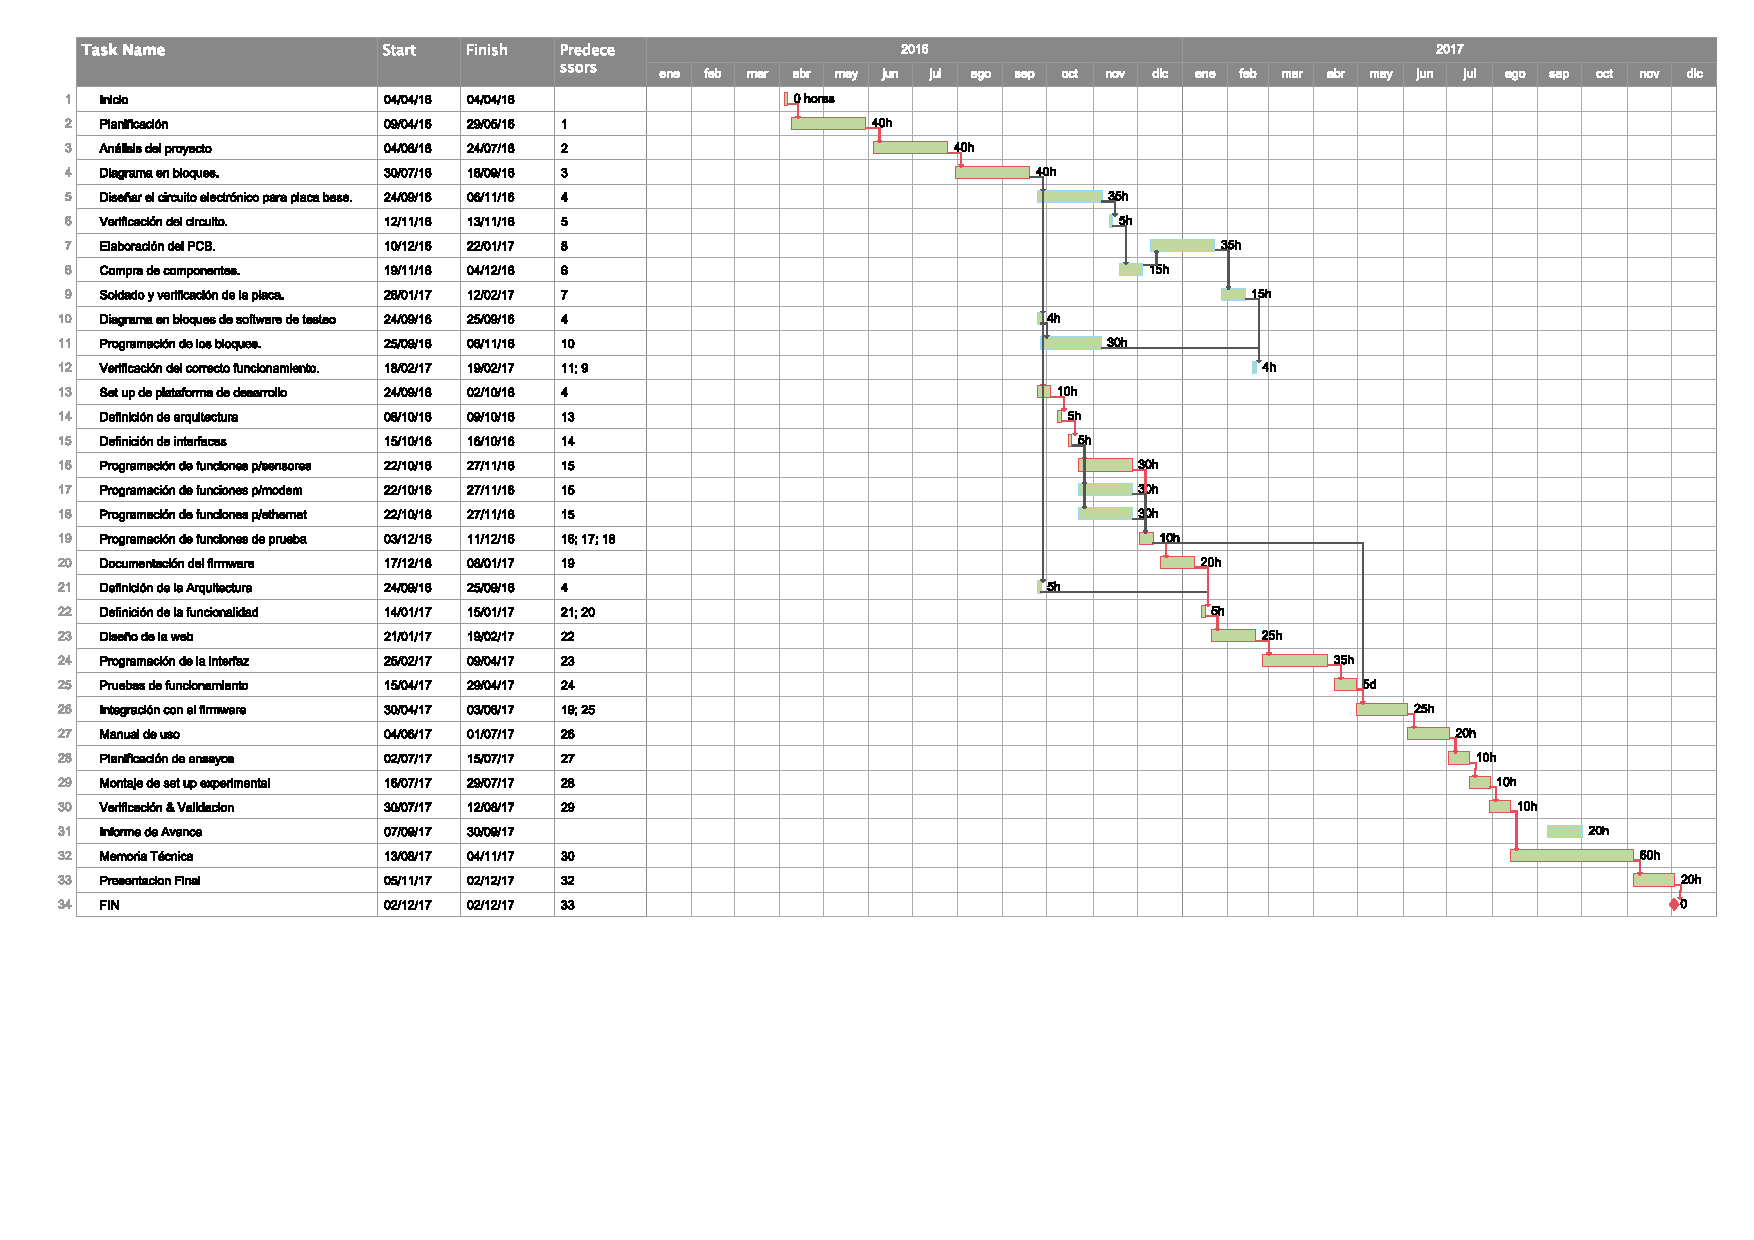
\includegraphics[page=1,clip, trim=0.5cm 5cm 0cm 0cm, width=1.70\textwidth]{./Figures/gantt.pdf}
      \caption{Listado de tareas, y plafinicacion de tiempos de la implementación.}
      \label{fig:gantt}
  \end{figure}
\end{landscape}


Pero debido a la falta de experiencia en determinados temas, que fueron más complejos de lo que se estimo. Es por ello que en la siguiente tabla \ref{tab:update_task}, se va a mostrar el tiempo real y cuales fueron las tareas que requirieron más tiempo de lo planificado.

\begin{table}[hp]
  \begin{tabular}{|c|c|c|c|c|}
    \hline
       &       & \multicolumn{2}{c|}{ Tiempo} & \%  \\ \cline{3-4}
    Nro& Tarea &  Estimado &  Real & a más \\
    \hline
    9 & Soldado y verificacion de la placa & 15h & 24 & 60 \\
    18 & Programacion de funciones p/ethernet & 30h & 50h & 66,7 \\
    23 & Programacion de funciones p/ethernet & 25h & 35h & 40 \\
    \hline \hline
  \end{tabular}
  \caption{Comparación tiempo planificado vs real.}
  \label{tab:update_task}
\end{table}

Con lo cual hay una diferencia de 39 horas a más de lo planificado. Siendo que para el desarrollo de todo el proyecto se habían estimado 617 horas podemos concluir que la estimación de los tiempos no estuvo mal. 
Dado que habían temas que no se conocian con profundiad y de haber sido crítica la fecha de entrega se hubiera buscando ayuda de otro programador para poder avanzar en forma paralela. 

%Si en el texto se hace alusión a diferentes partes del trabajo referirse a ellas como capítulo, sección o subsección según corresponda. Por ejemplo: ``En el capítulo \ref{Chapter1} se explica tal cosa'', o ``En la sección \ref{sec:ejemplo} se presenta lo que sea'', o ``En la subsección \ref{subsec:ejemplo} se discute otra cosa''.
%
%Entre párrafos sucesivos dejar un espacio, como el que se observa entre este párrafo y el anterior. Pero las oraciones de un mismo párrafo van en forma consecutiva, como se observa acá. Luego, cuando se quiere poner una lista tabulada se hace así:
%
%\begin{itemize}
%	\item Este es el primer elemento de la lista.
%	\item Este es el segundo elemento de la lista.
%\end{itemize}
%
%Notar el uso de las mayúsculas y el punto al final de cada elemento.
%
%Si se desea poner una lista numerada el formato es este:
%
%\begin{enumerate}
%	\item Este es el primer elemento de la lista.
%	\item Este es el segundo elemento de la lista.
%\end{enumerate}
%
%Notar el uso de las mayúsculas y el punto al final de cada elemento.
%
%\subsection{Este es el título de una subsección}
%\label{subsec:ejemplo}
%
%Se recomienda no utilizar \textbf{texto en negritas} en ningún párrafo, ni tampoco texto \underline{subrayado}. En cambio sí se sugiere utilizar \textit{texto en cursiva} donde se considere apropiado.
%
%Se sugiere que la escritura sea impersonal. Por ejemplo, no utilizar ``el diseño del firmware lo hice de acuerdo con tal principio'', sino ``el firmware fue diseñado utilizando tal principio''. En lo posible hablar en tiempo pasado, ya que la memoria describe un trabajo que ya fue realizado.
%
%Se recomienda no utilizar una sección de glosario sino colocar la descripción de las abreviaturas como parte del mismo cuerpo del texto. Por ejemplo, RTOS (\textit{Real Time Operating System}, Sistema Operativo de Tiempo Real) o en caso de considerarlo apropiado mediante notas a pie de página.
%
%Si se desea indicar alguna página web utilizar el siguiente formato de referencias bibliográficas, dónde las referencias se detallan en la sección de bibliografía de la memoria,utilizado el formato establecido por IEEE en \citep{IEEE:citation}. Por ejemplo, ``el presente trabajo se basa en la plataforma EDU-CIAA-NXP, la cual se describe en detalle en \citep{CIAA}''.
%
%\subsection{Figuras} 
%
%Al insertar figuras en la memoria se deben considerar determinadas pautas. Para empezar, usar siempre tipografía claramente legible. Luego, tener claro que es incorrecto escribir por ejemplo esto: ``El diseño elegido es un cuadrado, como se ve en la siguiente figura:''
%
%\begin{figure}[h]
%\centering
%
\includegraphics[scale=.35]{./Figures/cuadradoAzul.png}
%\end{figure}
%
%La forma correcta de utilizar una figura es la siguiente: ``Se eligió utilizar un cuadrado azul para el logo, el cual se ilustra en la figura \ref{fig:cuadradoAzul}''.
%
%\begin{figure}[h]
%	\centering
%	
\includegraphics[scale=.35]{./Figures/cuadradoAzul.png}
%	\caption{Ilustración del cuadrado azul que se eligió para el diseño del logo.}
%	\label{fig:cuadradoAzul}
%\end{figure}
%
%El texto de las figuras debe estar siempre en español, excepto que se decida reproducir una figura original tomada de alguna referencia. En ese caso la referencia de la cual se tomó la figura debe ser indicada en el epígrafe de la figura e incluida como una nota al pie, como se ilustra en la figura \ref{fig:palabraIngles}.
%
%\begin{figure}[h!]
%	\centering
%	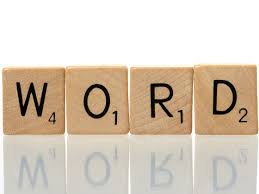
\includegraphics[scale=.25]{./Figures/word.jpeg}
%	\caption{Imagen tomada de la página oficial del procesador\protect\footnotemark.}
%	\label{fig:palabraIngles}
%\end{figure}
%
%\footnotetext{\url{https://goo.gl/images/i7C70w}}
%
%
%La figura y el epígrafe deben conformar una unidad cuyo significado principal pueda ser comprendido por el lector sin necesidad de leer el cuerpo central de la memoria. Para eso es necesario que el epígrafe sea todo lo detallado que corresponda y si en la figura se utilizan abreviaturas entonces aclarar su significado en el epígrafe o en la misma figura.
%
%\begin{figure}[h]
%	\centering
%	
\includegraphics[scale=.4]{./Figures/questionMark.png}
%	\caption{El lector no sabe por qué de pronto aparece esta figura.}
%	\label{fig:questionMark}
%\end{figure}
%
%Nunca colocar una figura en el documento antes de hacer la primera referencia a ella, como se ilustra con la figura \ref{fig:questionMark}, porque sino el lector no comprenderá por qué de pronto aparece la figura en el documento, lo que distraerá su atención.
%
%\subsection{Tablas}
%
%Para las tablas utilizar el mismo formato que para las figuras, sólo que el epígrafe se debe colocar arriba de la tabla, como se ilustra en la tabla \ref{tab:peces}. Observar que sólo algunas filas van con líneas visibles y notar el uso de las negritas para los encabezados.  La referencia se logra utilizando el comando \verb|\ref{<label>}| donde label debe estar definida dentro del entorno de la tabla.
%
%\begin{verbatim}
%\begin{table}[h]
%	\centering
%	\caption[caption corto]{caption largo más descriptivo}
%	\begin{tabular}{l c c}    
%		\toprule
%		\textbf{Especie}       & \textbf{Tamaño}  & \textbf{Valor aprox.}\\
%		\midrule
%		Amphiprion Ocellaris	  & 10 cm 			& \$ 6.000 \\		
%		Hepatus Blue Tang      & 15 cm			 & \$ 7.000 \\
%		Zebrasoma Xanthurus    & 12 cm			 & \$ 6.800 \\
%		\bottomrule
%		\hline
%	\end{tabular}
%	\label{tab:peces}
%\end{table}
%\end{verbatim}
%
%\begin{table}[h]
%	\centering
%	\caption[caption corto]{caption largo más descriptivo}
%	\begin{tabular}{l c c}    
%		\toprule
%		\textbf{Especie} 	 & \textbf{Tamaño}  & \textbf{Valor aprox.}  \\
%		\midrule
%		Amphiprion Ocellaris	 & 10 cm 			& \$ 6.000 \\		
%		Hepatus Blue Tang	 & 15 cm				& \$ 7.000 \\
%		Zebrasoma Xanthurus	 & 12 cm				& \$ 6.800 \\
%		\bottomrule
%		\hline
%	\end{tabular}
%	\label{tab:peces}
%\end{table}
%
%En cada capítulo se debe reiniciar el número de conteo de las figuras y las tablas, por ejemplo, Fig. 2.1 o Tabla 2.1, pero no se debe reiniciar el conteo en cada sección. Por suerte la plantilla se encarga de esto por nosotros.
%
%\subsection{Ecuaciones}
%\label{sec:Ecuaciones}
%
%Al insertar ecuaciones en la memoria estas se deben numerar de la siguiente forma:
%
%\begin{equation}
%	\label{eq:metric}
%	ds^2 = c^2 dt^2 \left( \frac{d\sigma^2}{1-k\sigma^2} + \sigma^2\left[ d\theta^2 + \sin^2\theta d\phi^2 \right] \right)
%\end{equation}
%                                                        
%Es importante tener presente que en el caso de las ecuaciones estas pueden ser referidas por su número, como por ejemplo ``tal como describe la ecuación \ref{eq:metric}'', pero también es correcto utilizar los dos puntos, como por ejemplo ``la expresión matemática que describe este comportamiento es la siguiente:''
%
%\begin{equation}
%	\label{eq:schrodinger}
%	\frac{\hbar^2}{2m}\nabla^2\Psi + V(\mathbf{r})\Psi = -i\hbar \frac{\partial\Psi}{\partial t}
%\end{equation}
%
%Para las ecuaciones se debe utilizar un tamaño de letra equivalente al utilizado para el texto del trabajo, en tipografía cursiva y preferentemente del tipo Times New Roman o similar. El espaciado antes y después de cada ecuación es de aproximadamente el doble que entre párrafos consecutivos del cuerpo principal del texto. Por suerte la plantilla se encarga de esto por nosotros.
%
%Para generar la ecuación \ref{eq:metric} se utilizó el siguiente código:
%
%\begin{verbatim}
%\begin{equation}
%	\label{eq:metric}
%	ds^2 = c^2 dt^2 \left( \frac{d\sigma^2}{1-k\sigma^2} + 
%	\sigma^2\left[ d\theta^2 + 
%	\sin^2\theta d\phi^2 \right] \right)
%\end{equation}
%\end{verbatim}
%
%Y para la ecuación \ref{eq:schrodinger}:
%
%\begin{verbatim}
%\begin{equation}
%	\label{eq:schrodinger}
%	\frac{\hbar^2}{2m}\nabla^2\Psi + V(\mathbf{r})\Psi = 
%	-i\hbar \frac{\partial\Psi}{\partial t}
%\end{equation}
%
%\end{verbatim}
 
	\chapter{Diseño e Implementación} % Main chapter title

\label{Chapter3} % Change X to a consecutive number; for referencing this chapter elsewhere, use \ref{ChapterX}
\definecolor{mygreen}{rgb}{0,0.6,0}
\definecolor{mygray}{rgb}{0.5,0.5,0.5}
\definecolor{mymauve}{rgb}{0.58,0,0.82}

\lstset{ %
  backgroundcolor=\color{white},   % choose the background color; you must add \usepackage{color} or \usepackage{xcolor}
  basicstyle=\footnotesize,        % the size of the fonts that are used for the code
  breakatwhitespace=false,         % sets if automatic breaks should only happen at whitespace
  breaklines=true,                 % sets automatic line breaking
  captionpos=b,                    % sets the caption-position to bottom
  commentstyle=\color{mygreen},    % comment style
  deletekeywords={...},            % if you want to delete keywords from the given language
  %escapeinside={\%*}{*)},          % if you want to add LaTeX within your code
  %extendedchars=true,              % lets you use non-ASCII characters; for 8-bits encodings only, does not work with UTF-8
  %frame=single,	                   % adds a frame around the code
  keepspaces=true,                 % keeps spaces in text, useful for keeping indentation of code (possibly needs columns=flexible)
  keywordstyle=\color{blue},       % keyword style
  language=[ANSI]C,					% the language of the code
  %otherkeywords={*,...},           % if you want to add more keywords to the set
  numbers=left,                    % where to put the line-numbers; possible values are (none, left, right)
  numbersep=5pt,                   % how far the line-numbers are from the code
  numberstyle=\tiny\color{mygray}, % the style that is used for the line-numbers
  rulecolor=\color{black},         % if not set, the frame-color may be changed on line-breaks within not-black text (e.g. comments (green here))
  showspaces=false,                % show spaces everywhere adding particular underscores; it overrides 'showstringspaces'
  showstringspaces=false,          % underline spaces within strings only
  showtabs=false,                  % show tabs within strings adding particular underscores
  stepnumber=1,                    % the step between two line-numbers. If it's 1, each line will be numbered
  stringstyle=\color{mymauve},     % string literal style
  tabsize=2,	                   % sets default tabsize to 2 spaces
  title=\lstname,                   % show the filename of files included with \lstinputlisting; also try caption instead of title
  morecomment=[s]{/*}{*/}%
}


%----------------------------------------------------------------------------------------
%	SECTION 1
%----------------------------------------------------------------------------------------
En este capítulo se presenta cómo se desarrolló el hardware básico para simular el entorno de funcionamiento y cómo fue implementado el firmware.
%La idea de esta sección es resaltar los problemas encontrados, los criterios utilizados y la justificación de las decisiones que se hayan tomado.
%Se puede agregar código o pseudocódigo dentro de un entorno lstlisting con el siguiente código:

\section{Hardware}

Primeramente se diseñó un circuito electrónico que permite simular el entorno de funcionamiento de una bodega. Para ello se utilizó lo aprendido a la largo del curso de \emph{diseño de PCBs en KICAD}. 

En la figura \ref{fig:diagrama_sistema} se aprecia el entorno de trabajo del sistema. El mismo interactua con una bomba de agua que permite llevar desde el deposito del liquido refrigerante a los tanques que están en proceso de fermentación.
Recibiendo como información la temperatura de los tanques, el equipo debe controlar la bomba y la electroválvula correspondiente. De esta forma controlada la temperatura acorde a los parámetros definidos por el usuario. 


\begin{figure}[!htb]
  \centering
  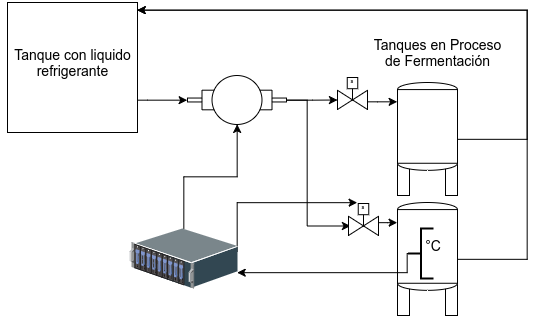
\includegraphics[scale=0.7]{./Figures/diagrama_del_sistema.png}
  \caption{Entorno del sistema de control del equipo.}
  \label{fig:diagrama_sistema}
\end{figure}

\subsection{ Módulos requeridos}
Para llevar a cabo el proyecto, se dividió el sistema en los siguientes módulos:
\begin{description}
  \item[Módem:] sera el encargado de transmitir las alertas mediante SMS utilizando el modulo SIM800L.
  \item[Actuadores:] salidas que permiten controlar la bomba y electroválvulas. Debido a que se utilizo la CIAA-NXP esto ya está resuelto.
  \item[Sensores:] entradas que permitan simular el comportamiento de los sensores, para esto se utilizaron potenciómetros.
  \item[CPU:] unidad encargada de controlar el funcionamiento del sistema. Incorporada en la placa CIAA-NXP. 
\end{description}

\subsection{Características del hardware}

La placa diseñada que va a reemplazar el entorno del sistema que se vió en la figura \ref{fig:diagrama_sistema} por el sitema que está compuesto por el modem y circuitos electronicos que permiten:
\begin{itemize}
  \item Simular el estado de la temperatura
  \item Adaptar los niveles de tensión.
  \item Mostrar el estado de los actuadores.
  \item Conectar el módem GPRS.
\end{itemize}

    La forma de conexión con la CIAA-NXP se muesetra en la figura \ref{fig:diagrama_simulado}.

\begin{figure}[!htb]
  \centering
  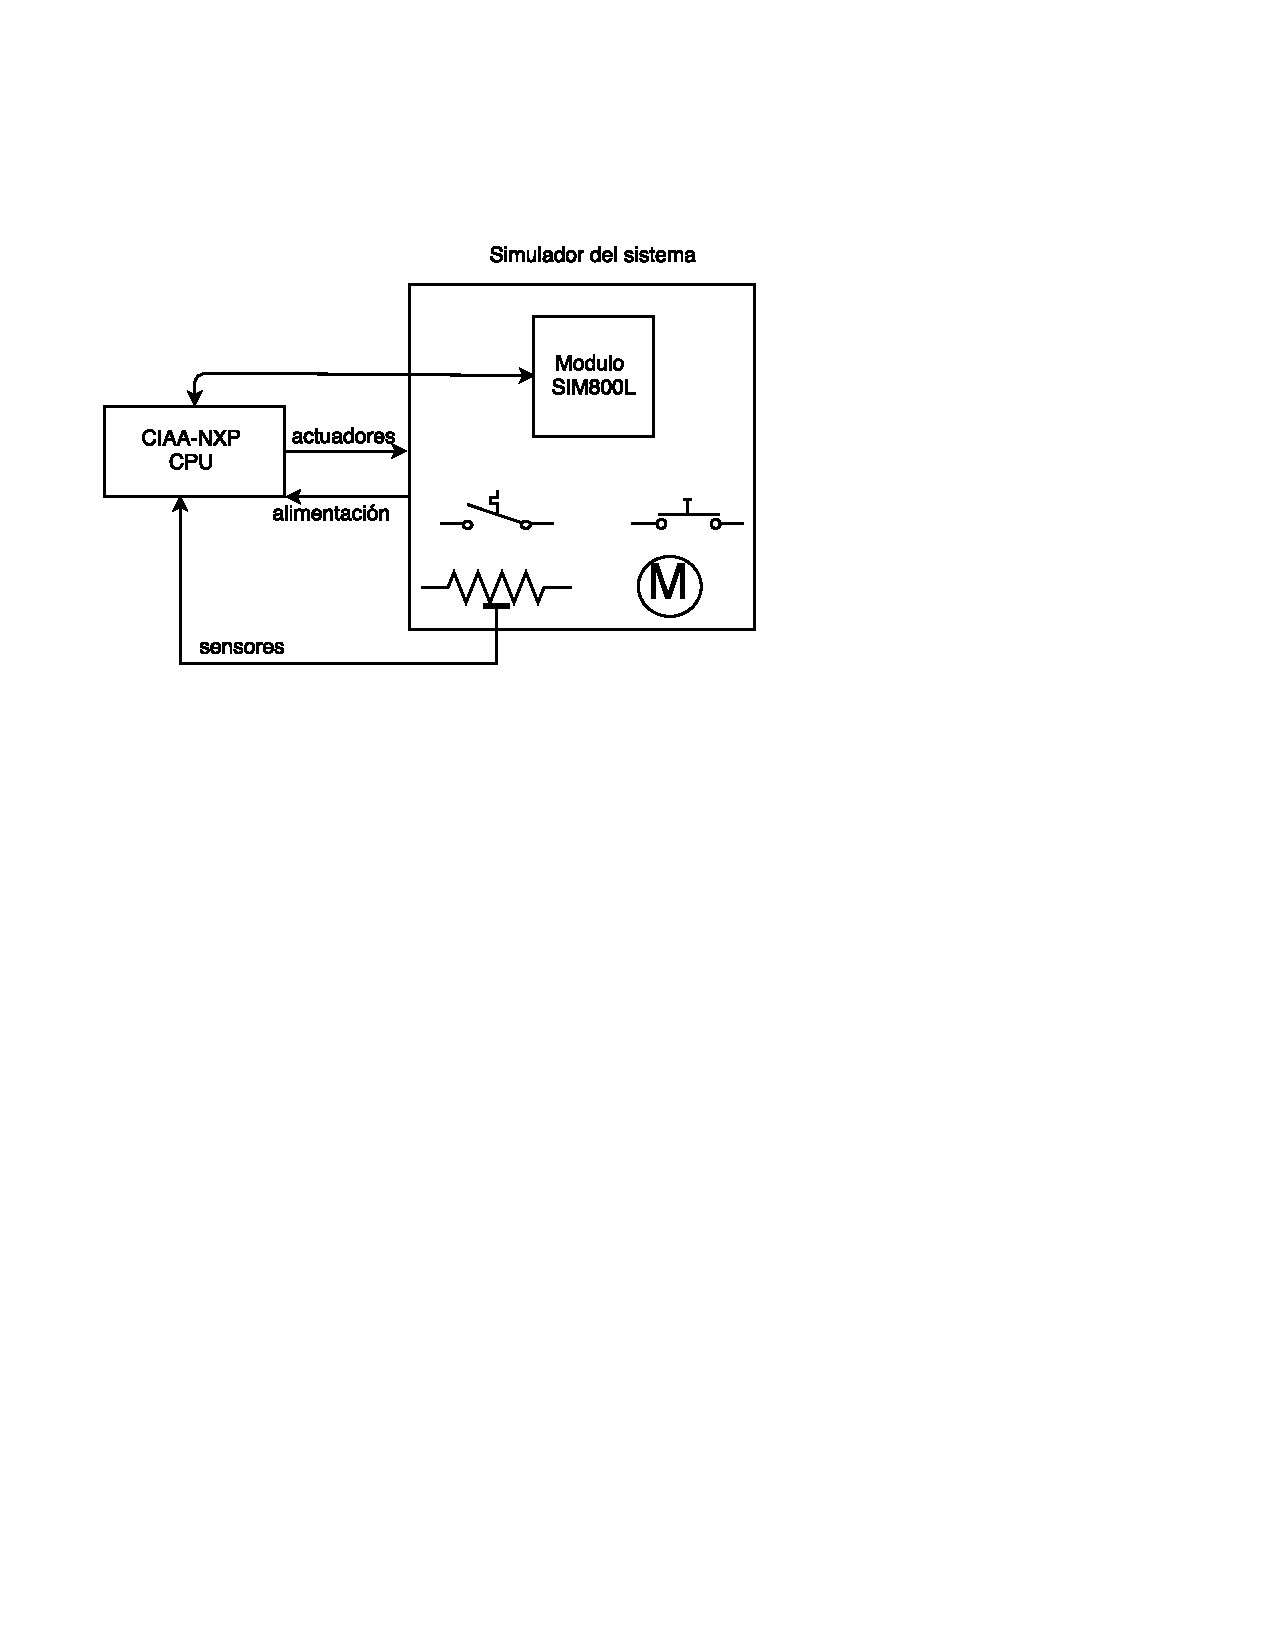
\includegraphics[page=1,scale=1,clip,trim=1.5cm 16.5cm 5.5cm 3.5cm]{./Figures/ciaa_placa_base.pdf}
  \caption{Entorno del sistema de control del equipo.}
  \label{fig:diagrama_simulado}
\end{figure}


Los especificaciones de la placa de simulación son:

\begin{itemize}
  \item 1 Salida con regulación de corriente, para simular sensores de 4mA a 20mA.
  \item 1 Salida con tensión variable, utilizando el regulador LM317.
  \item 1 Salida del sensor de temperatura LM35.
  \item 2 Salidas con tensión variable, utilizando potenciómetros. 
  \item 4 Entradas digitales conectadas a leds.
  \item 4 Salidas conectadas a pulsadores. 
  \item 1 Zócalo para la conexión del modulo SIM800L. 
  \item 1 salida de 5V a 3A y otra de 3.3V a 1A. 
\end{itemize}

El módulo SIM800L que se muestra en la figura \ref{fig:sim800l}, es un módem GPRS que cuenta con las siguientes especificaciones:

\begin{figure}[!htb]
  \centering
  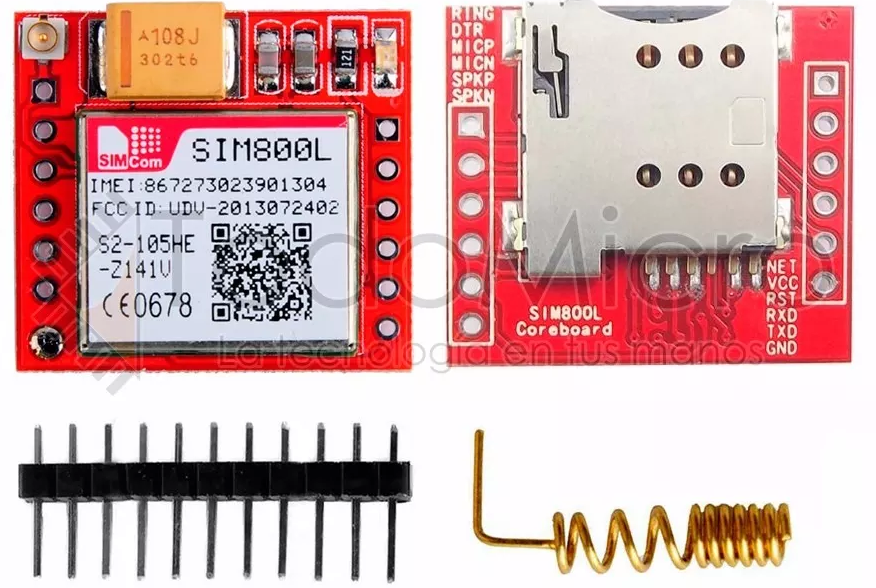
\includegraphics[scale=0.2]{./Figures/sim800.png}
  \caption{Módem SIM800L.}
  \label{fig:sim800l}
\end{figure}

\begin{itemize}
  \item Alimentación: 3.4V a 4.4V (4.0V recomendado)
  \item  CuatriBanda 850/900/1800/1900MHz
  \item  GPRS Multi Slot class 8/10
  \item  Control mediante comandos AT (GSM 07.07 ,07.05 y comandos AT SIMCOM).
\end{itemize}


En la figura \ref{fig:essim800} se puede apreciar el esquemático implementado para la conexión del módem GSM. Éste requiere adaptar los niveles de tensión para interactuar con la CIA-NXP, para el cual se utilizó el max3232.
\begin{figure}[!hp]
  \centering
  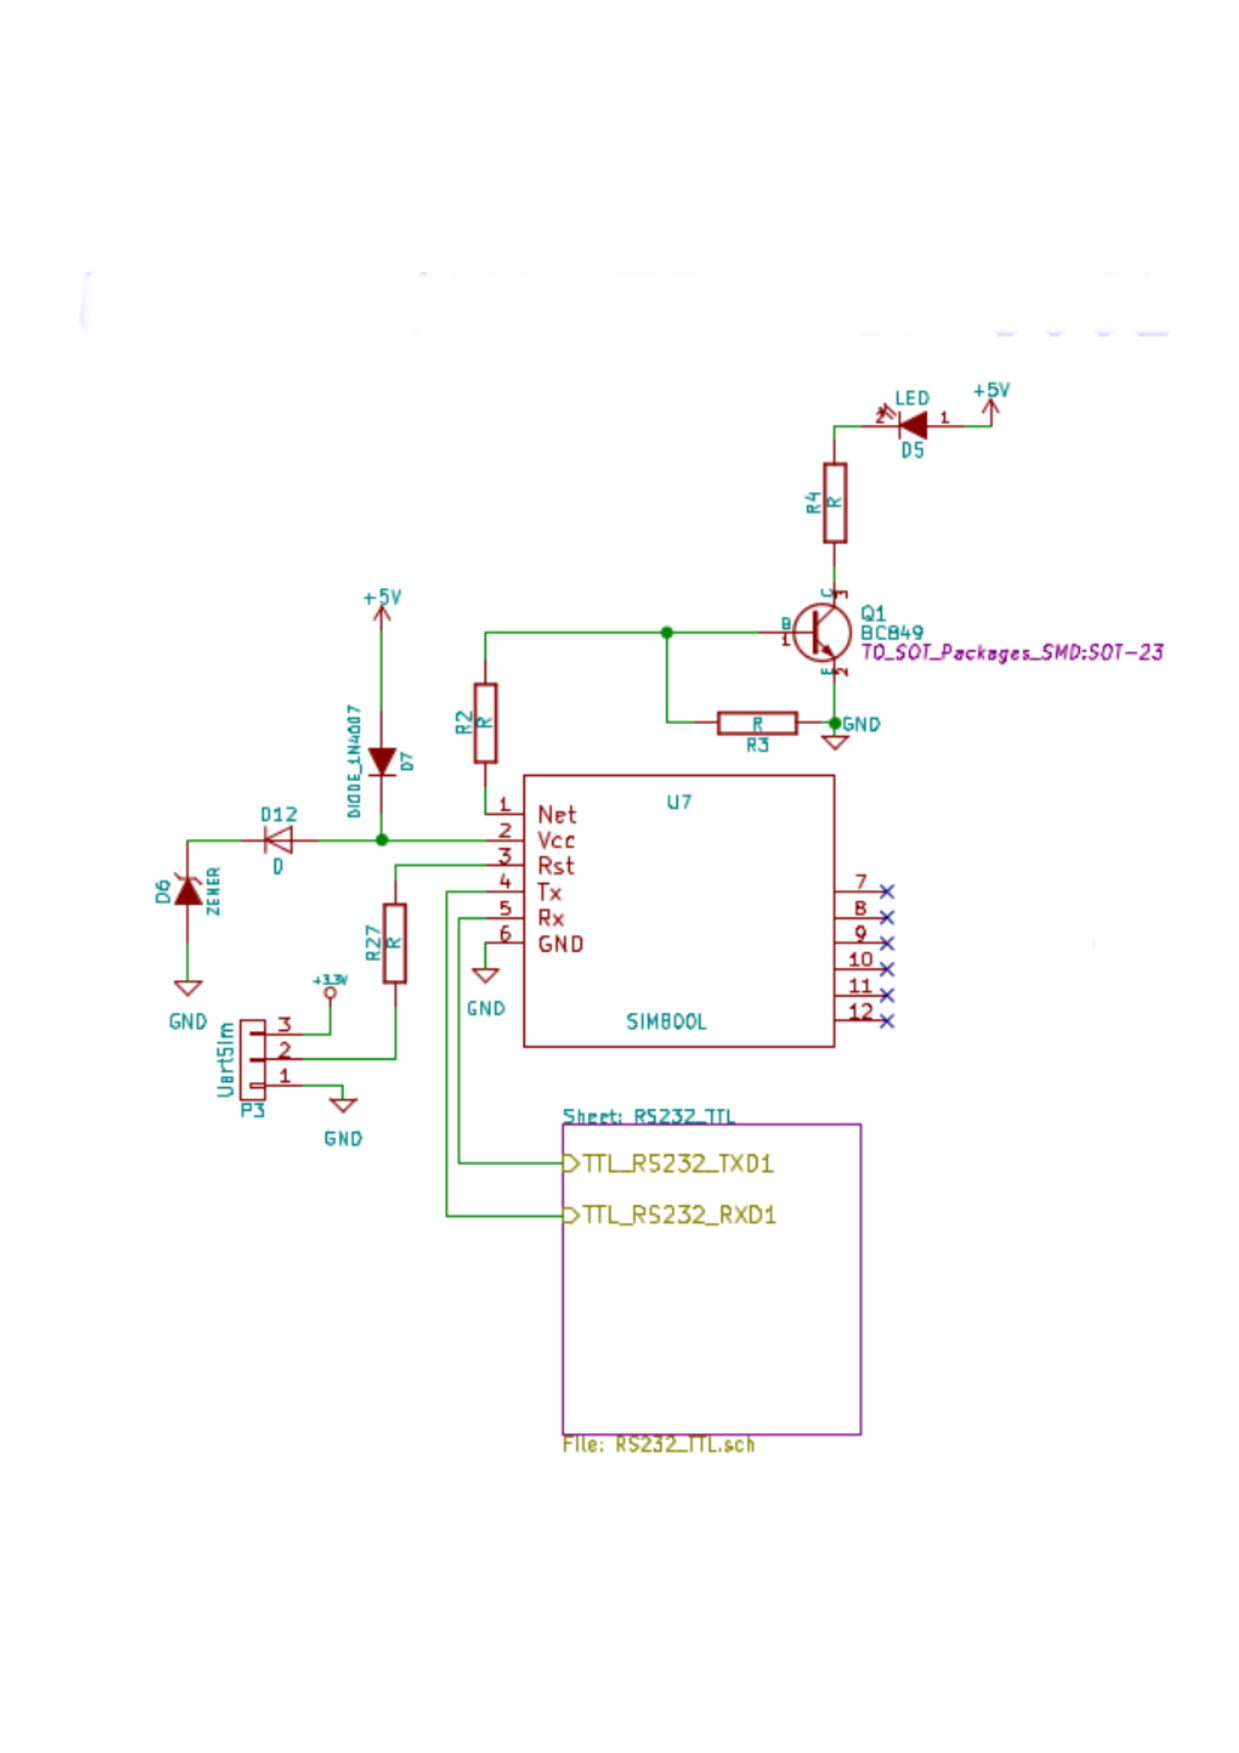
\includegraphics[page=1,scale=0.5,clip,trim=1cm 4.7cm 1.2cm 2.5cm]{./Figures/sch_modem_sim800.pdf}
  \caption{Módulo SIM800l e índice de esquemáticos.}
  \label{fig:essim800}
\end{figure}

Para la alimentación del circuito se utilizó el regulador LM2576. El mismo se tomó de la nota de aplicación \citep{Texas:LM2576}.
Para regular a 3.3V se utilizó el integrado LM11733 circuito extraído de la nota de aplicación \citep{Texas:LM11733}.
\begin{figure}[!hp]
  \centering
  \includegraphics[page=3,scale=0.7,angle=270,clip,trim=2cm 3cm 6.5cm 2.5cm]{./Figures/schematic.pdf}
  \caption{Fuente de alimentación DC/DC.}
  \label{fig:fuente}
\end{figure}

Para lograr la simulación de distintos tipos de sensores, se utilizaron circuitos como el que se muestra en la figura \ref{fig:temp_tens}  que permiten generar corrientes de 4mA a 20mA. También reguladores de tensión, y hasta un sensor de temperatura. Para estos circuitos se utilizaron las notas de aplicación de Texas Instruments\citep{Texas:LM317} - capitulo 8 páginas 12 y 13 y sensor temperatura: \citep{Texas:LM35} - 8.2.1 Basic Centigrade Temperature Sensor. 
\begin{figure}[!hp]
  \centering
  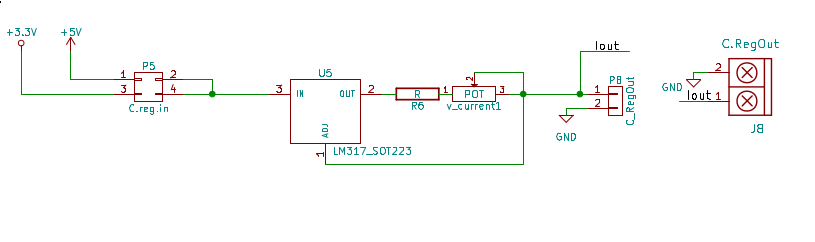
\includegraphics[scale=0.5]{./Figures/sch_ireg.png}
  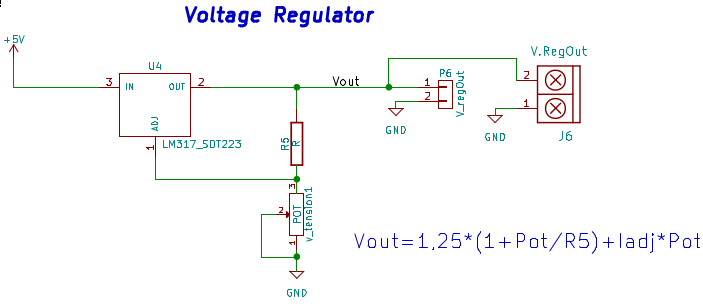
\includegraphics[scale=0.5]{./Figures/sch_vreg.png}
  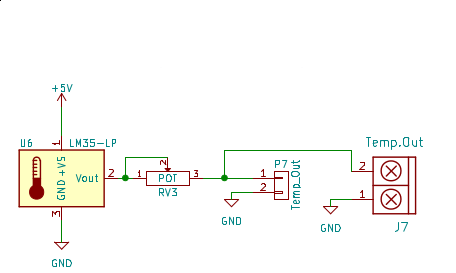
\includegraphics[scale=0.5]{./Figures/sch_lm35.png}
  \caption{Regulador de corriente, de tensión y del sensor de temperatura.}
  \label{fig:temp_tens}
\end{figure}

Para concluir, se utilizaron unos circuitos básicos que permiten interactuar en forma simple con el sistema y realizar pruebas de funcionamiento. Los mismos fueron extraídos del esquemático utilizado en el proyecto de la EDU-CIA \footnote{\url{http://www.proyecto-ciaa.com.ar/devwiki/lib/exe/fetch.php?media=desarrollo:edu-ciaa:edu-ciaa-nxp:edu-ciaa-nxp\_color.pdf}}, figura \ref{fig:pul_leda_pulses}.


\begin{figure}[!hp]
  \begin{subfigure}{0.4\textwidth}
    \centering
    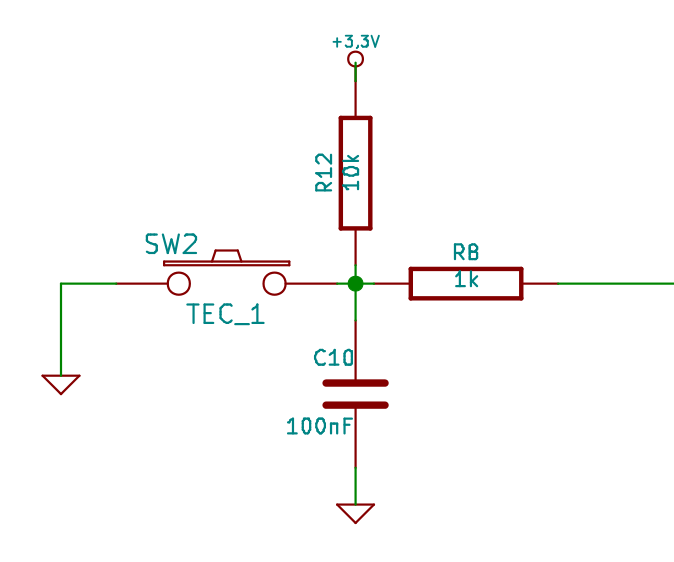
\includegraphics[width=1\linewidth]{./Figures/pulse_sch.png}
    \caption{Circuito de los pulsadores.}
  \end{subfigure}%
  \hfill
  \begin{subfigure}{0.4\textwidth}
    \centering
    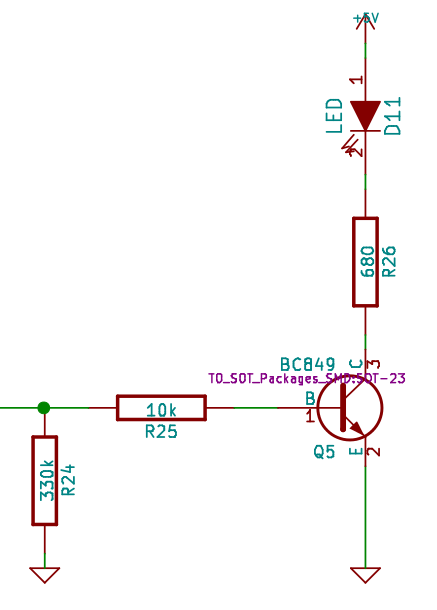
\includegraphics[width=1\linewidth]{./Figures/led_sch.png}
    \caption{Circuito de los leds.}
  \end{subfigure}
  \caption{Esquematicos extraidos de la EDU-CIAA.}
  \label{fig:pul_leda_pulses}
\end{figure}

Con los esquemáticos terminados, se pasó a la elaboración del PCB. Los cuales se presentan en las siguientes figuras \ref{fig:layer_sup}, \ref{fig:layer_inf} y \ref{fig:pcb3d}.
\begin{figure}[!hp]
  \centering
  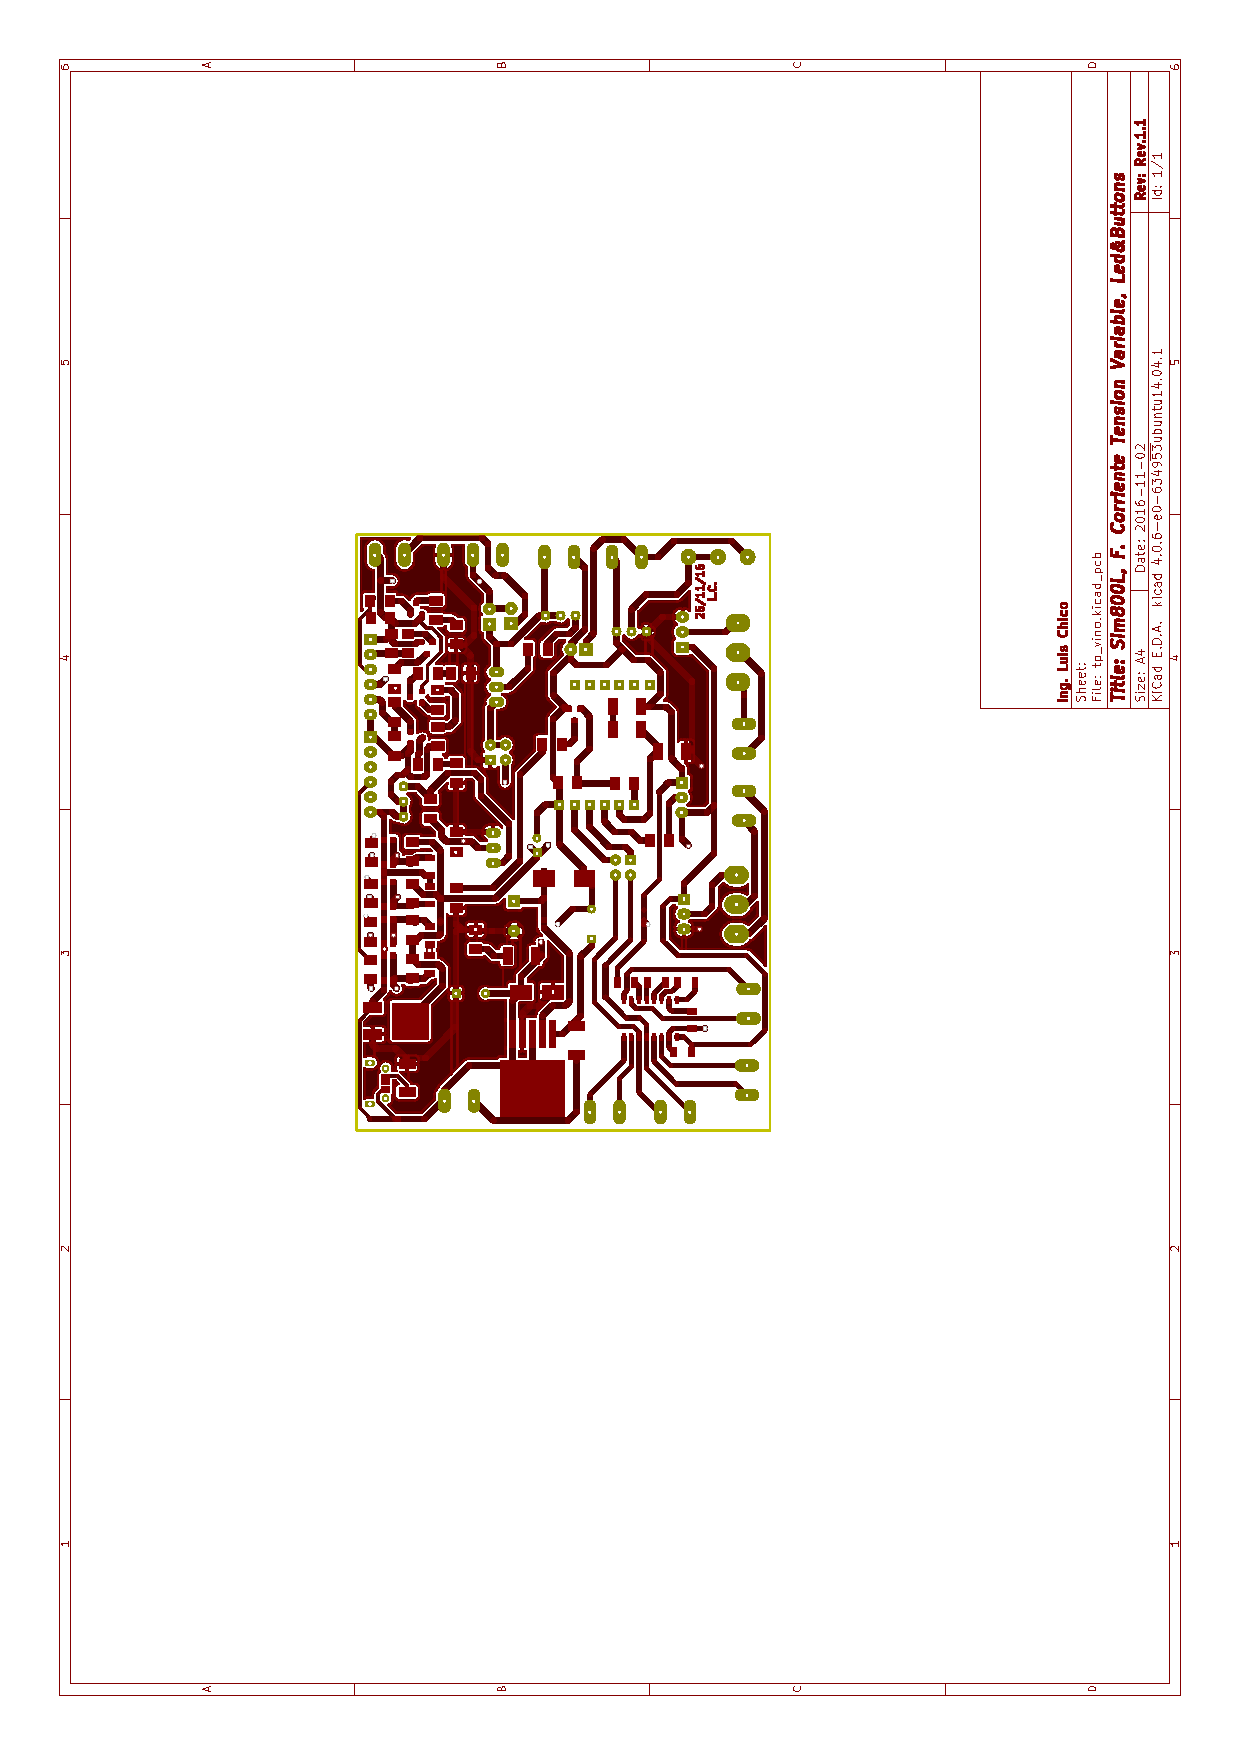
\includegraphics[page=1,angle=270,clip,trim=5.5cm 10cm 7.7cm 8.5cm]{./Figures/pcb_layer.pdf}
  \caption{Capa superior de la placa simulador de sensores.}
  \label{fig:layer_sup}
\end{figure}
\begin{figure}[!hp]
  \centering
  \includegraphics[page=2,angle=270,clip,trim=5.5cm 10cm 7.7cm 8.5cm]{./Figures/pcb_layer.pdf}
  \caption{Capa inferior de la placa simulador de sensores.}
  \label{fig:layer_inf}
\end{figure}

\begin{figure}[!hp]
  \centering
  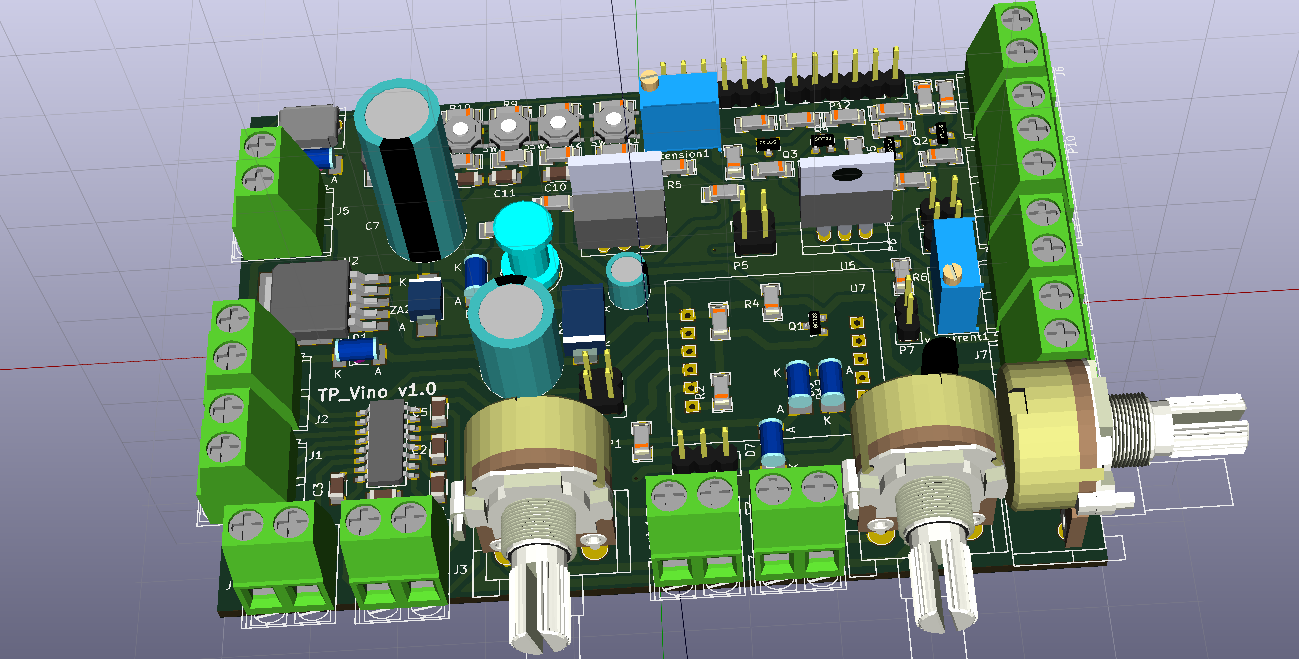
\includegraphics[scale=0.3]{./Figures/pcb_3d.png}
  %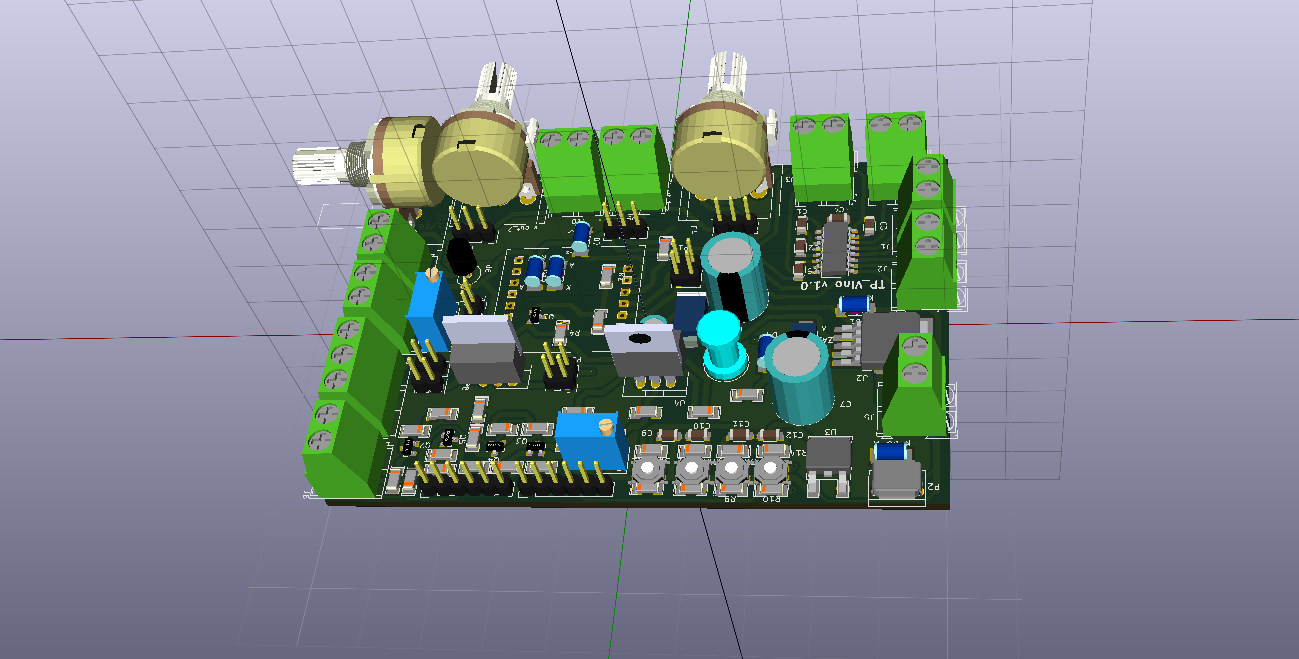
\includegraphics[scale=0.3]{./Figures/pcb_3d_back.png}
  \caption{Placa simulador de sensores 3D.}
  \label{fig:pcb3d}
\end{figure}

No obstante, por cuestiones de tiempo no se llegó a implementar la placa que se deiseñó del simulador del sistema. Y se terminó desarrollando una placa experimental que permitió realizar las primeras pruebas y que se presenta en la figura \ref{fig:placa_básicafirst}.

\begin{figure}[!ht]
  \centering
  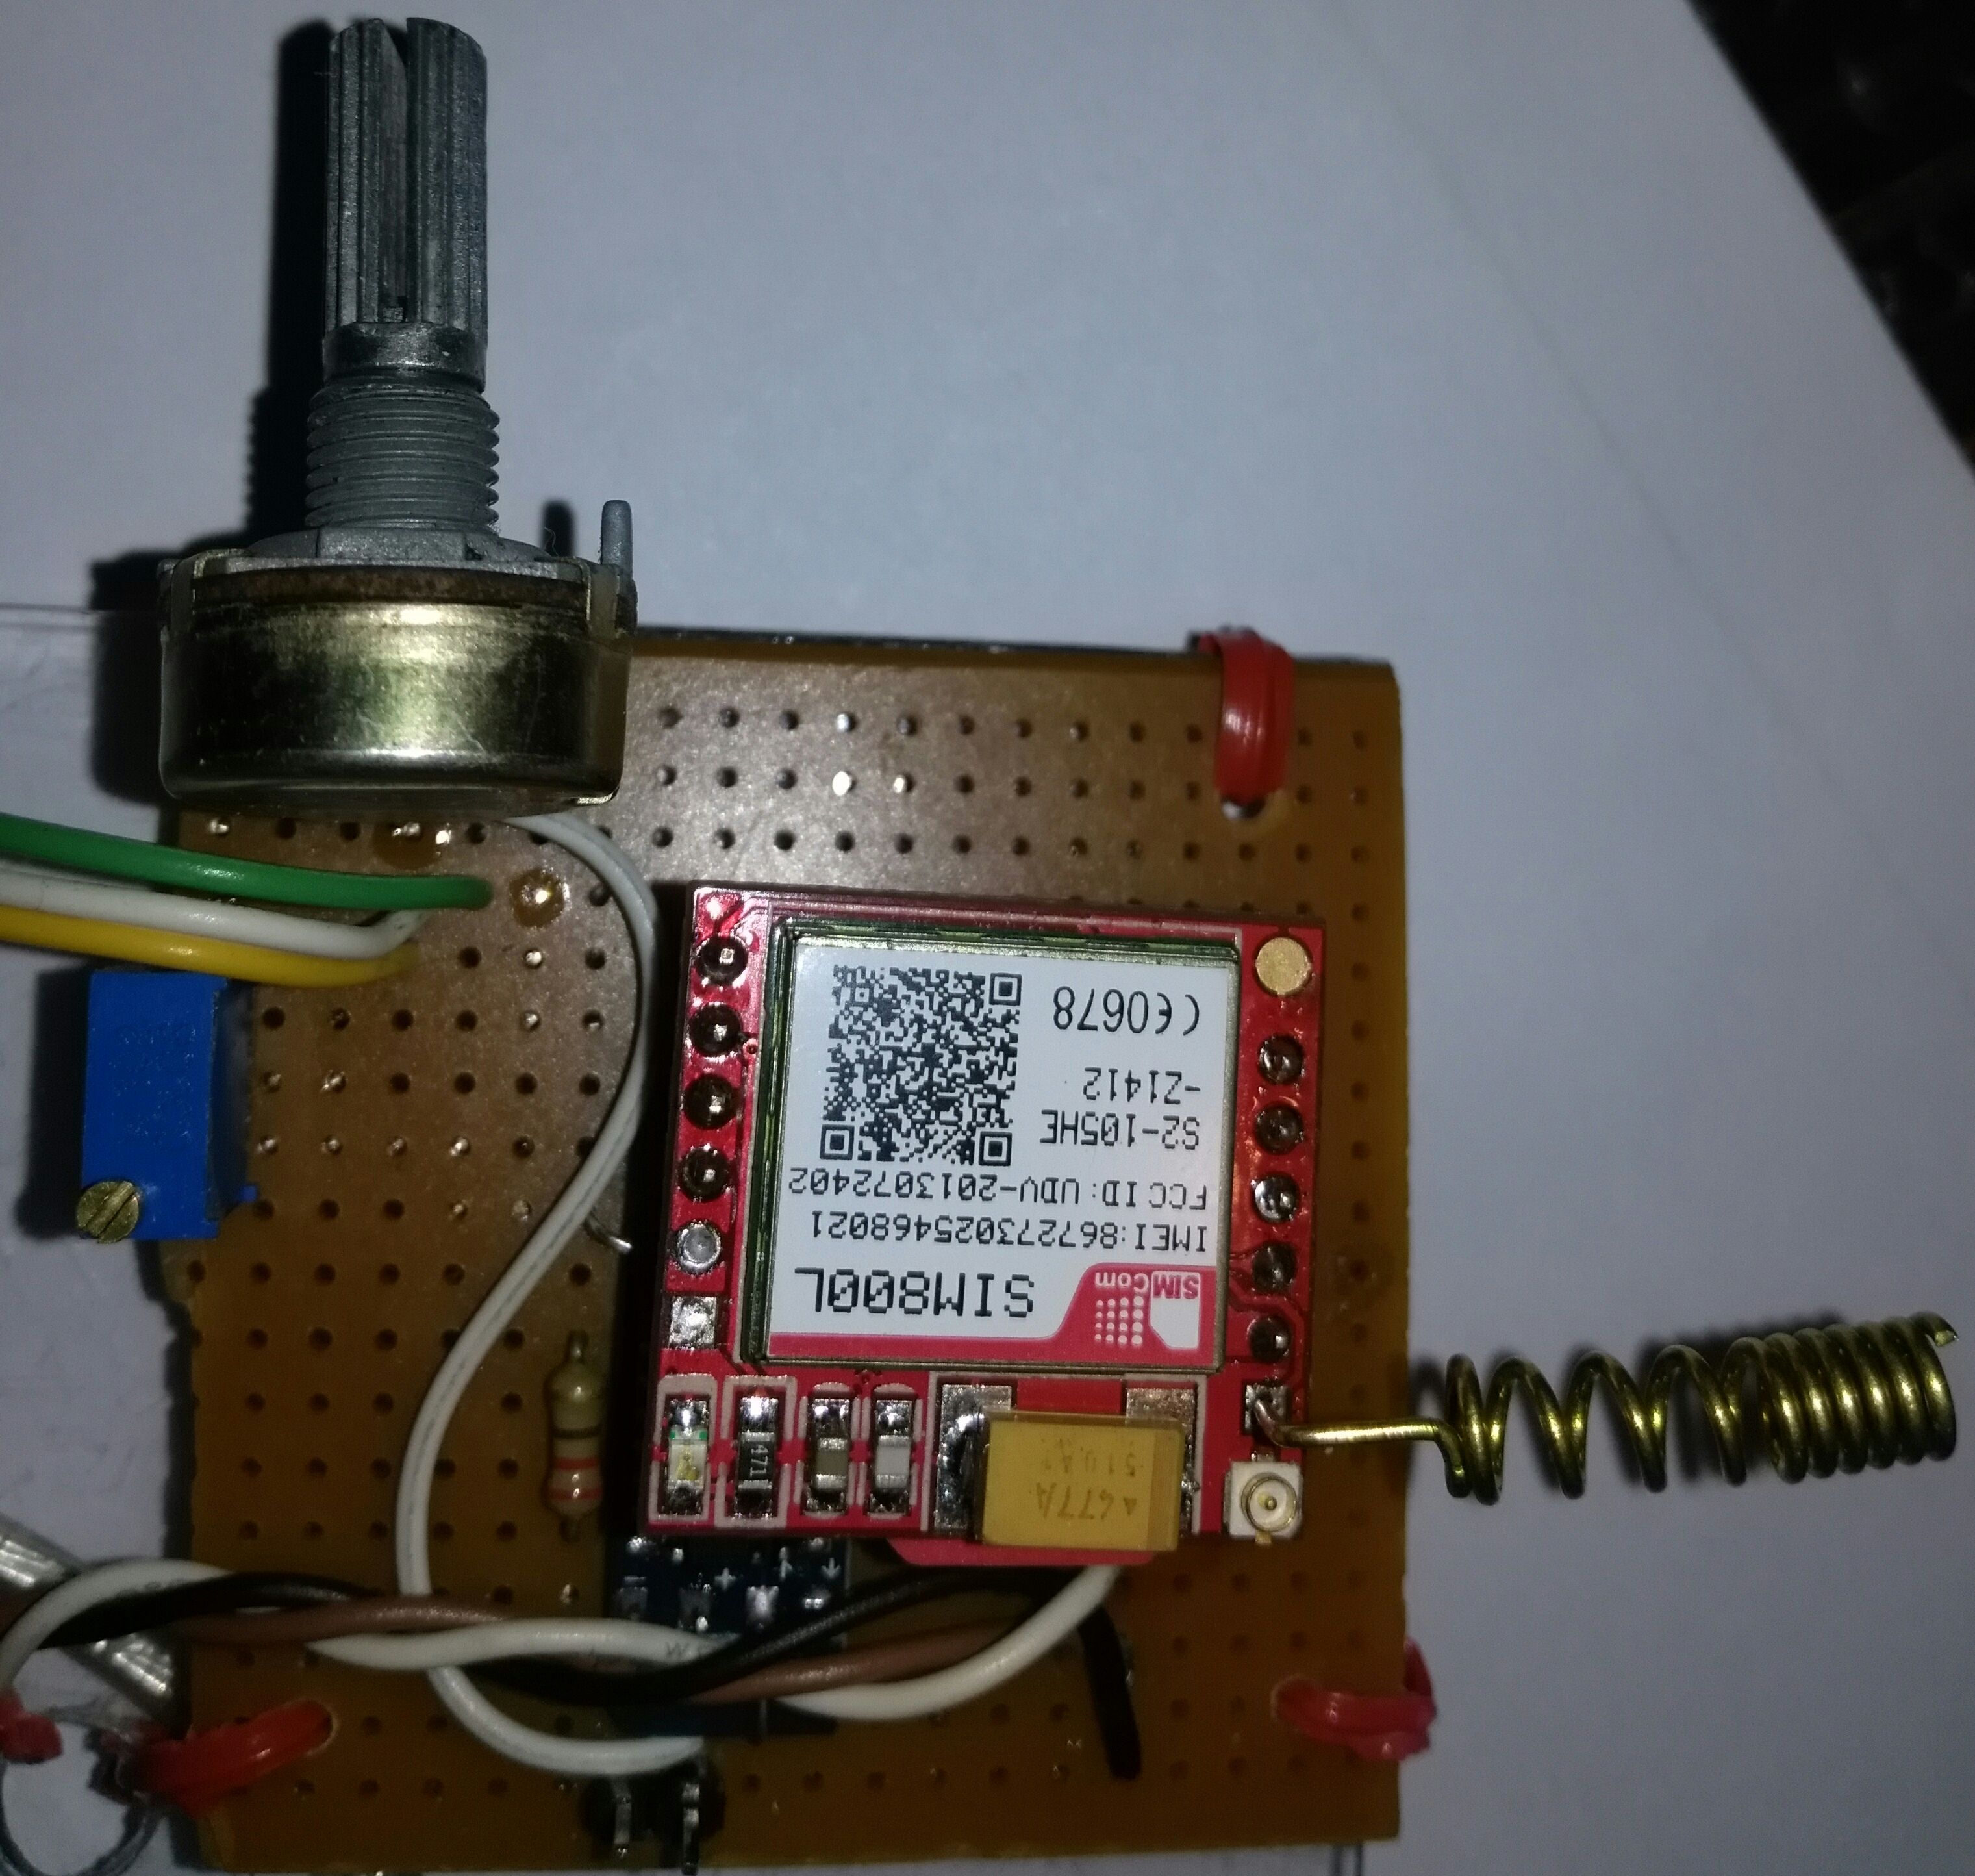
\includegraphics[scale=.07]{./Figures/placa_basica.jpg}
  \caption{Placa de simulación de temperatura y estado de la batería con el modulo SIM800L integrado.}
  \label{fig:placa_básicafirst}
\end{figure}


%Dado que por falta de tiempo no se elaboro el PCB diseñado, pero se realizó una versión simplificada del mismo que se verá más adelante. 
%
%Surgieron varios imprevistos, principalmente con el modulo SIM800L, el cual posee grandes inconvenientes a la hora de detectar la SIM. Luego de una serie de búsquedas en internet, donde muchos habían tenido un problema similar dado que:
%\begin{itemize}
%  \item La fuente de alimentación fue subdimensionada.
%  \item Módulo es muy sensible y se debe limpiar bien los contactos de la SIM.
%  \item O problemas con las soldaduras del módulo.
%\end{itemize}
%Finalmente, como el módulo ya había sido comprado y se encontró la falla a tiempo, se utilizó este en el prototipo.
%Pero este no se recomienda por los problemas mencionados anteriormente. A futuras implementación este módulo será reemplazado.




\section{Software}
\subsection{Aplicación}
Se dividieron las tareas en tres módulos:
\begin{itemize}
  \item Módem 
  \item Control
  \item Sensores
\end{itemize}

\subsection*{Módem}

\begin{minipage}{0.4\textwidth}
    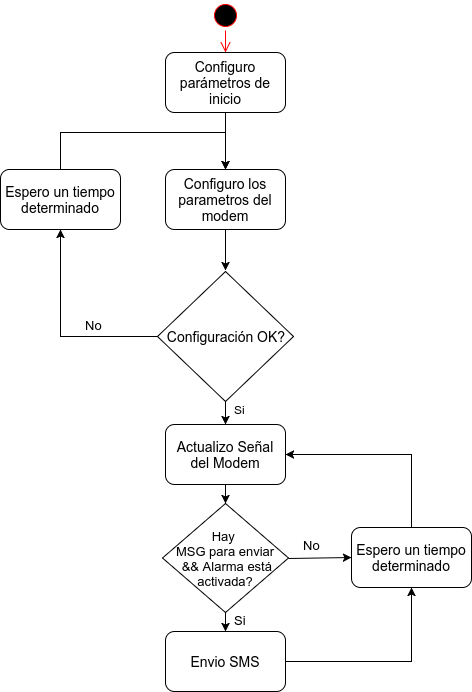
\includegraphics[width=\textwidth]{./Figures/modem_task.png}
\end{minipage}\hspace{5mm} %
\begin{minipage}{0.6\textwidth}
  En esta tarea se inicializa las configuraciones iniciales para el uso del módem. Es la encargada de interactuar con el módulo GPRS, realizando consultas del estado de señal y de enviando los mensajes de alarmas en caso de ser necesarios.

 En el diagrama de flujo de la izquierda se ve como fue implementado.
\end{minipage}

\subsection*{Control}
Con esta tarea se analiza el resultado los sensores de temperatura, y de la batería. Se verifica que estén dentro de los parámetros configurados por el usuario y se actúa en consecuencia. Siendo que el sitema de control actua cuando: la temperatura del sistema excede la máxima configurada, este procede a encender la bomba para que circule el líquido refrigerante y la electroválvula correspondiente. Luego una vez que el sistema llega a la temperatura mínima, este deshabilita la bomba y la electroválvula.

También es la encargada de setear los actuadores según sean especificados en la plataforma web.

La implementación se puede apreciar en la figura \ref{fig:control_task}.
\begin{figure}[!hp]
  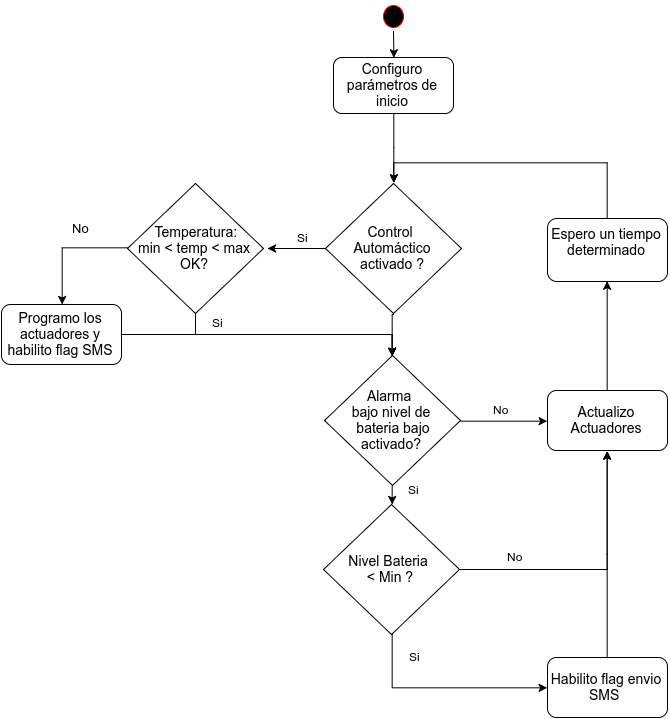
\includegraphics[scale=.5]{./Figures/control_task.png}
  \caption{Diagrama de flujo de la tarea de control.}
  \label{fig:control_task}
\end{figure}

\subsection*{Sensor}
\begin{minipage}{0.4\textwidth}
  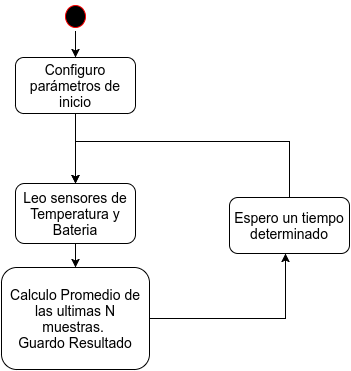
\includegraphics[width=\linewidth,scale=.5]{./Figures/sensor_task.png}
\end{minipage}\hspace{5mm} %
\begin{minipage}{0.6\textwidth}
Esta consulta el estado de los sensores y calcula el promedio de las ultimas N muestras. Este es el valor que utiliza la tarea de control para definir si es necesario encender los actuadores correspondientes o apagarlos.

El diagrama de flujo se puede apreciar la izquierda.
\end{minipage}

\subsection{ Plataforma web}
Mediante la plataforma web diseñada se busca que el usuario pueda ver los datos de los sensores, tener control sobre los actuadores y realizar las configuraciones necesarias. 

Para poder realizarlo, fue necesario profundizar los siguientes temas:
\begin{description}
  \item[HTML:] La página web se desarrolló en este lenguaje, permite darle la estructura básica y se realiza sobre texto plano, es decir no se requiere ninguna aplicación adicional simplemente un editor de texto. Luego es el navegador web quien tiene la tarea de interpretarlo. 
  \item[CSS:] Mediante este código se realiza la presentación de la página, permitiendo así modificar la visualización de la misma y darle un formato mas profesional y elegante.
  \item[SVG:] Mediante este lenguaje se implementaron los gráficos correspondientes para mostrar los resultados de los sensores y el estado de los actuadores.
  \item[AJAX:] es un recurso muy utilizado cuando se desarrollan web en sistemas embebidos. Permite actualizar el estado de la web sin tener que consultar todo el contenido, simplemente se descarga una primera vez y luego se realizan consultas de los valores que quieren actualizar. 
  \item[SSI:] Si bien la implementación que ofrece FreeRTOS es reducida. Es más que suficiente para poder agregar contenido a nuestra pagina en forma dinámica.
  \item[CGI:] Por medio de este el cliente que navegar por nuestra plataforma puede enviar y solicitar datos, al servidor.
\end{description}

\subsection*{Diseño web}
Al iniciar el diseño de la web, no tenía experiencia previa. Es por ello que se inició buscando información en internet, donde se encontraron varias páginas con cursos de HTML, CSS, y AJAX que son de forma online y gratuita. Las que mas se utilizó fueron:
\begin{itemize}
  \item \url{https://www.w3schools.com}
  \item \url{https://es.khanacademy.org}
  \item \url{https://www.codecademy.com}
\end{itemize}
con lo cual se logro una primera versión de la web, como se puede ver en la figura \ref{fig:old_web}.
\begin{figure}[!htb]
  \centering
  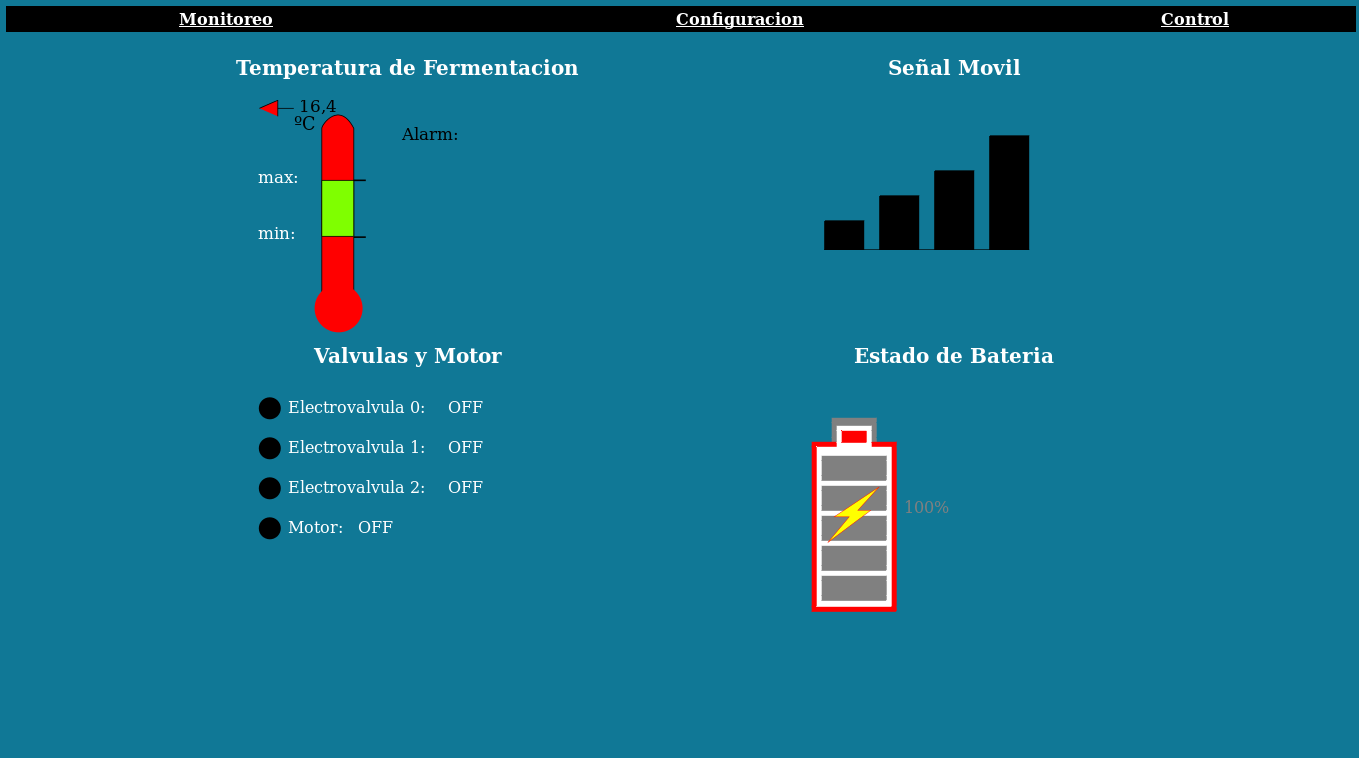
\includegraphics[scale=.25]{./Figures/old_web.png}
  \caption{Primera versión de la web de monitoreo.}
  \label{fig:old_web}
\end{figure}

Cuando ya estaba funcionando en forma correcta, se paso a mejorar las presentación de la misma. Para ello se usó un témplate que se ajustara a las necesidades, es decir mediante un archivo que contiene un estilo ya predefinido modifica la apariencia de la web. Pudiendo ver dicho cambio en la siguiente figura \ref{fig:web_monitoreo}.

\begin{figure}[!h]
  \centering
  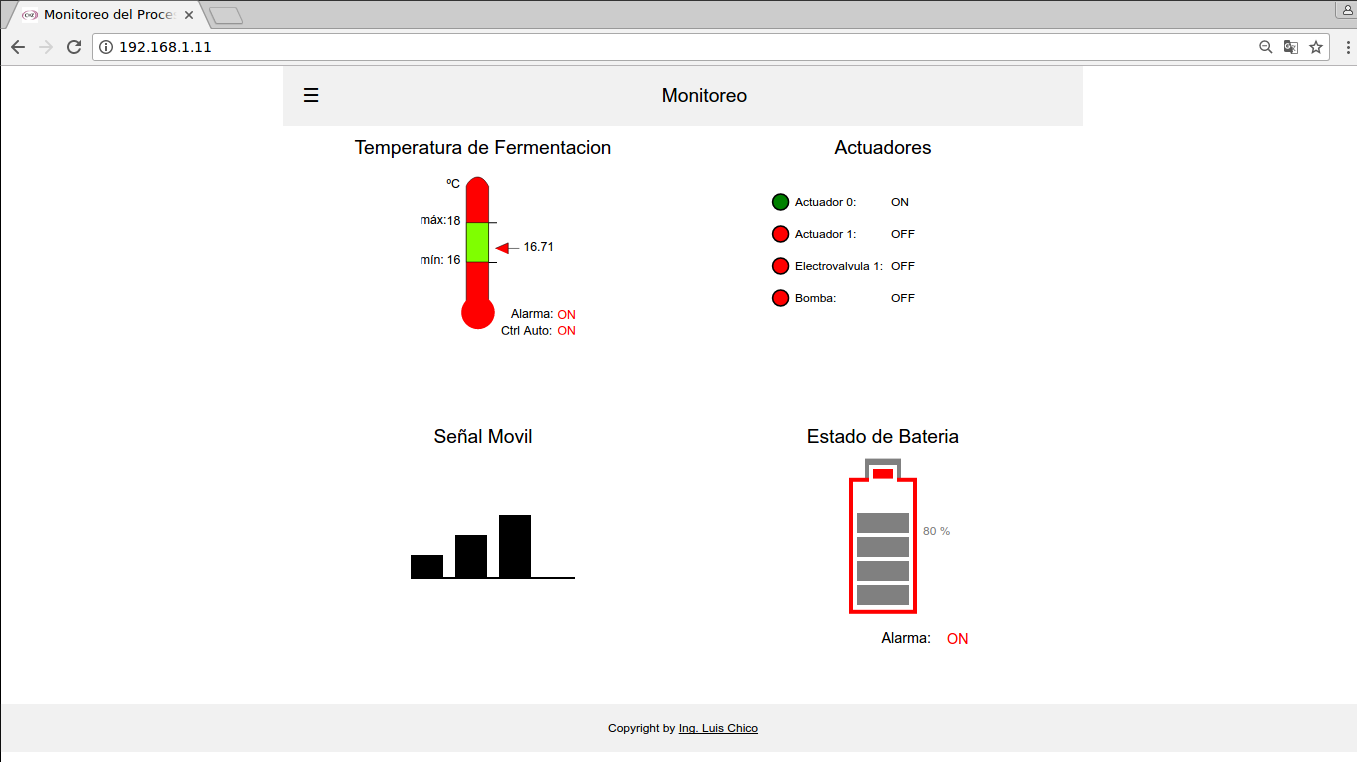
\includegraphics[scale=.25]{./Figures/web_monitoreo.png}
  \caption{Versión actualizada haciendo uso del témplate.}
  \label{fig:web_monitoreo}
\end{figure}

Este template fue encontrando en w3school\footnote{\url{https://www.w3schools.com/w3css/w3css_templates.asp}}. Siendo que cumplía los siguientes requerimientos:
\begin{itemize}
  \item Sea amigable.
  \item Compatibles con distintos navegadores, especialmente los más utilizados como ser: Google-Chrome y Firefox. 
  \item Sea cómodo de navegar en distintos dispositivos, como tablets, celulares y PCs.
\end{itemize}


\subsection*{Configuración del servidor}
Al iniciar el servidor debemos tener en cuenta que este sera el encargado de gestionar las peticiones del usuario. Es decir una vez que el usuario ingresa la dirección del servidor, este le transmite la información de la web.  Para realizar la comunicación entre cliente y servidor, se utilizo la API de lwIP  que utiliza una serie de callbacks para controlar los eventos debido a la comunicación de la red. Es por ello que para optimizar los recursos se utilizo AJAX, permitiendo que el cliente sea el encargado de realizar las consultas al server en forma periódica. La información se solicita mediante directivas del tipo SSI.
Es decir, solo se transmite un archivo ajax.shtml con los parámetros que se van a actualizar. Luego el navegador, mediante una serie de funciones en JavaScript es el encargado de actualizar los cambios realizados.  
Podemos ver el procedimiento mencionado en la siguiente figura\footnote{\url{http://laboratorios.fi.uba.ar/lse/tesis/LSE-FIUBA-Trabajo-Final-CESE-Patricio-Bos-2016.pdf}, figura 3.9.} \ref{fig:ajax_sec}.
\begin{figure}[!htb]
  \centering
  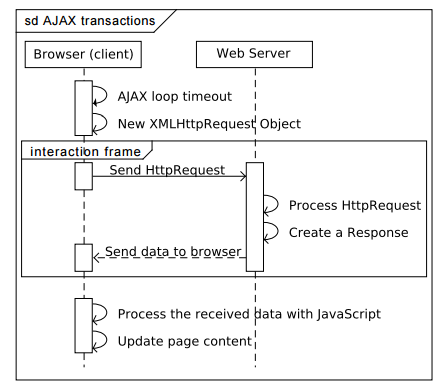
\includegraphics[scale=.8]{./Figures/ajax_sec.png}
  \caption{Diagrama de secuencia AJAX.}
  \label{fig:ajax_sec}
\end{figure}


La configuración establecida por default es la que se muestra en la siguiente Tabla \ref{tab:servercfg}.

\begin{table}[!h]
  \centering
  \begin{tabular}{l c}
    \hline 
    Parámetro    & Valor \\
    \hline \hline
    IP               & 192.168.1.11 \\
    Mascara de red   & 255.255.255.0 \\
    Puerta de enlace & 192.168.0.1 \\
    Puerto           & 80 \\
    DHCP             & Deshabilitado \\
    \hline
  \end{tabular}
  \caption{Configuración por default del servidor}
  \label{tab:servercfg}
\end{table}



\section{Diseño del sistema web embebido}
Se procede a navegar por el menú, figura \ref{fig:web_menus_num}, para constatar que todo el sistema esta funcionando en forma correcta. Al presionar donde dice menú, se puede configurar lo siguiente:

\begin{figure}[h]
  \centering
  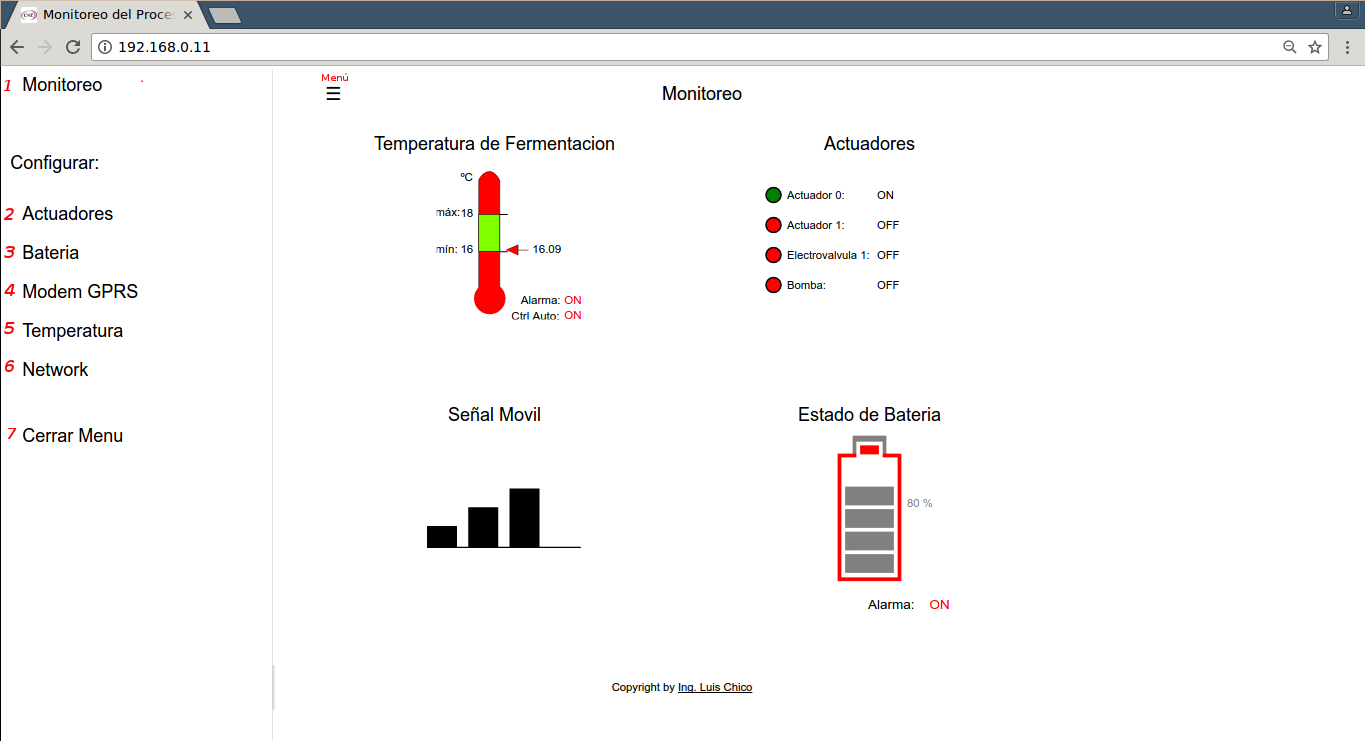
\includegraphics[scale=.25]{./Figures/web_menus_num.png}
  \caption{Opciones del al presionar sobre el menú desplegable.}
  \label{fig:web_menus_num}
\end{figure}

\begin{description}
  \item[1. Monitoreo:] Dirige a la pantalla principal, donde ver el estado del sistema. figura \ref{fig:web_monitoreo}.
  \item[2. Actuadores:] setear en forma manual el estado de los mismos. figura \ref{fig:web_act}.
  \item[3. Batería:] Aquí se podrá setear la alarma debido al nivel de descarga de batería. Esta enviará un SMS indicando que se alcanzó dicho estado. figura \ref{fig:web_bat}.
  \item[4. Módem GPRS:] En este menú podremos configurar 2 personas a quienes serán enviadas las alertas debido al accionar de alguna alarma, figura \ref{fig:web_Modem}.
  \item[5. Temperatura:] Aquí se configura el rango de temperatura, la alarma correspondiente y si se activa el control automático de la misma. De estar activado, actuará en forma automática sobre la bomba y la electroválvula para mantener la temperatura dentro de dicho rango. figura \ref{fig:web_temp}.
  \item[6. Network:] Aquí se configura los parámetros de la red, IP, mascara de red y puerta de enlace. figura \ref{fig:cfg_net}.
  \item[7. Cerrar Menú:] Esta opción cierra el menú, permitiendo quitar las opciones de menú.
\end{description}

\begin{figure}[h]
  \centering
  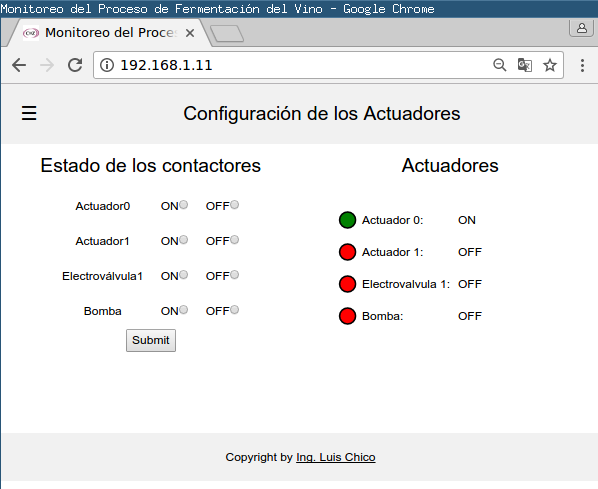
\includegraphics[scale=.35]{./Figures/config_act.png}
  \caption{ Activar/Desactivar actuadores.}
  \label{fig:web_act}
\end{figure}

\begin{figure}[h]
  \centering
  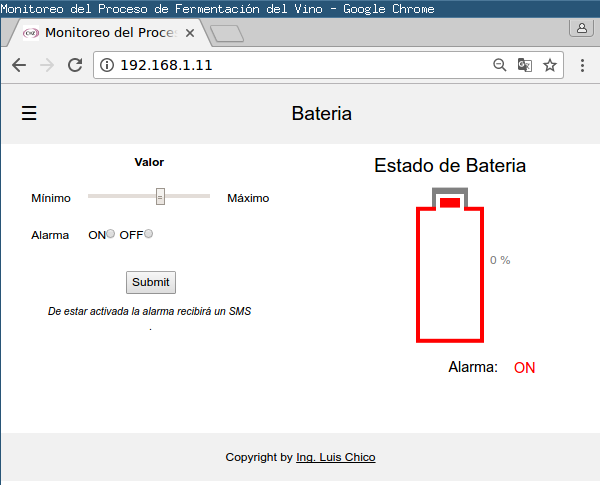
\includegraphics[scale=.35]{./Figures/config_bat.png}
  \caption{Configurar nivel de descarga para accionar la alerta por batería baja.}
  \label{fig:web_bat}
\end{figure}
\begin{figure}[h]
  \centering
  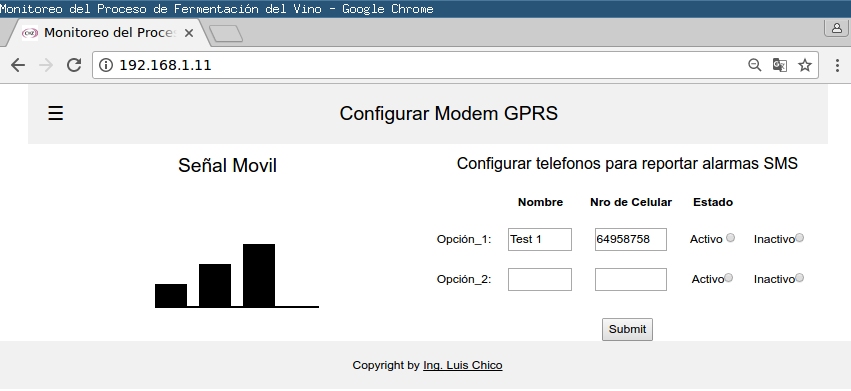
\includegraphics[scale=.35]{./Figures/config_Modem.png}
  \caption{Configuración de los celulares.}
  \label{fig:web_Modem}
\end{figure}
\begin{figure}[h]
  \centering
  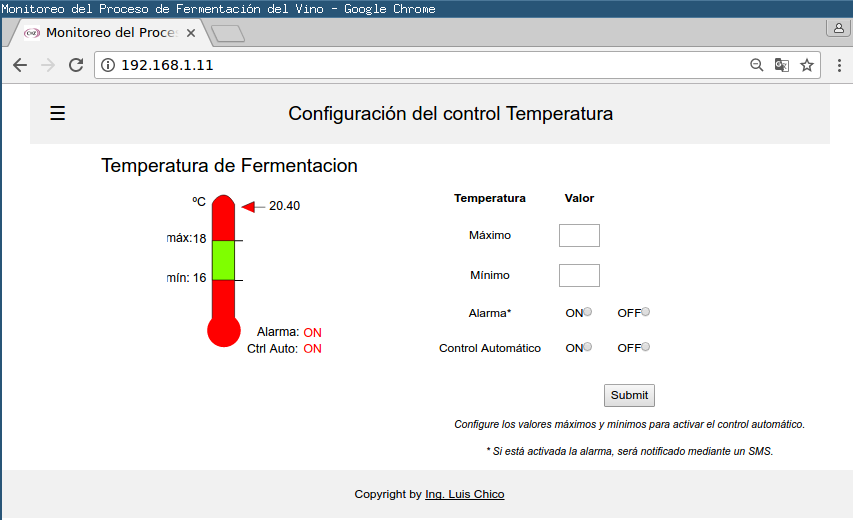
\includegraphics[scale=.35]{./Figures/config_temp.png}
  \caption{Configuración del rango de temperatura y activación del estado de control automático y alarma.}
  \label{fig:web_temp}
\end{figure}
\begin{figure}[h]
  \centering
  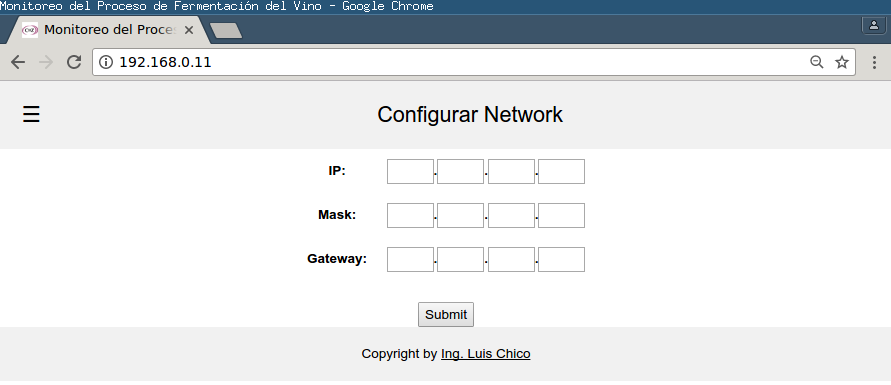
\includegraphics[scale=.35]{./Figures/config_network.png}
  \caption{Configuración de IP, mascara de red y puerta de enlace.}
  \label{fig:cfg_net}
\end{figure}











%\begin{verbatim}
%\begin{lstlisting}[caption= "un epígrafe descriptivo"]
%
%	las líneas de código irían aquí...
%	
%\end{lstlisting}
%\end{verbatim}
%
%A modo de ejemplo:
%
%\begin{lstlisting}[caption=Pseudocódigo del lazo principal de control.]  % Start your code-block
%
%#define MAX_SENSOR_NUMBER 3
%#define MAX_ALARM_NUMBER  6
%#define MAX_ACTUATOR_NUMBER 6
%
%uint32_t sensorValue[MAX_SENSOR_NUMBER];		
%FunctionalState alarmControl[MAX_ALARM_NUMBER];	//ENABLE or DISABLE
%state_t alarmState[MAX_ALARM_NUMBER];						//ON or OFF
%state_t actuatorState[MAX_ACTUATOR_NUMBER];			//ON or OFF
%
%void vControl() {
%
%	initGlobalVariables();
%	
%	period = 500 ms;
%		
%	while(1) {
%
%		ticks = xTaskGetTickCount();
%		
%		updateSensors();
%		
%		updateAlarms();
%		
%		controlActuators();
%		
%		vTaskDelayUntil(&ticks, period);
%	}
%}
%\end{lstlisting}
%



	% Chapter Template

\chapter{Ensayos y Resultados} % Main chapter title

\label{Chapter4} % Change X to a consecutive number; for referencing this chapter elsewhere, use \ref{ChapterX}

%----------------------------------------------------------------------------------------
%	SECTION 1
%----------------------------------------------------------------------------------------

\section{Pruebas funcionales del hardware}
\label{sec:pruebasHW}

La idea de esta sección es explicar cómo se hicieron los ensayos, qué resultados se obtuvieron y analizarlos.
 
	% Chapter Template

\chapter{Conclusiones} % Main chapter title

\label{Chapter5} % Change X to a consecutive number; for referencing this chapter elsewhere, use \ref{ChapterX}


%----------------------------------------------------------------------------------------

%----------------------------------------------------------------------------------------
%	SECTION 1
%----------------------------------------------------------------------------------------

\section{Conclusiones generales }

La idea de esta sección es resaltar cuáles son los principales aportes del trabajo realizado y cómo se podría continuar. Debe ser especialmente breve y concisa. Es buena idea usar un listado para enumerar los logros obtenidos.

%----------------------------------------------------------------------------------------
%	SECTION 2
%----------------------------------------------------------------------------------------
\section{Próximos pasos}

Acá se indica cómo se podría continuar el trabajo más adelante.
 
\end{verbatim}

Los apéndices también deben ir en archivos .tex separados y se deben ubicar dentro de la carpeta \emph{Appendices}. Los apéndices vienen comentados con el caracter \code{\%} por defecto y para incluirlos se debe eliminar dicho caracter.

Luego del preambulo, los capítulos y los apéndices, finalmente viene la bibliografía. El estilo bibliográfico (llamado \option{authoryear}) es utilizado por \LaTeX{} para generar las referencias y es un estilo con todas las características necesarias para su composición.  No se debe subestimar lo agradecido que estarán sus lectores al encontrar que las referencias se encuentran a un clic de distancia.  Por supuesto, esto depende de que usted haya puesto la url correspondiente en el archivo BibTex en primer lugar.

%----------------------------------------------------------------------------------------






